%%
%
% ARQUIVO: main.tex
%
% VERSÃO: 1.0
% DATA: Maio de 2016
% AUTOR: Coordenação de Trabalhos Especiais SE/8
% 
%  Arquivo tex principal do documento de Projeto de Fim de Curso (PFC).
%  Este arquivo SÓ PRECISA SER MODIFICADO NA PARTE DE CONTEÚDO:
%
%    a. colocar um \include{•} para cada capítulo do documento de PFC.
%
%%

% -----
% CLASSE DO DOCUMENTO DE P.FC
% -----
\documentclass{pfc}

% -----
% PACOTES LATEX USADOS NO DOCUMENTO DE PFC
% -----
\usepackage[brazilian]{babel}
\usepackage[utf8]{inputenc}
\usepackage[T1]{fontenc}

\usepackage{amsmath}
\usepackage{graphicx}
\usepackage{tabularx}
\usepackage{float}
\usepackage{color}
\usepackage{amsfonts,amssymb}
\usepackage[authoryear]{natbib}

\usepackage{enumitem}
\usepackage{rotating}
\usepackage{lipsum}
\usepackage{lastpage}
\usepackage{stringstrings}
\usepackage{pgffor}
\usepackage{pdftexcmds}
\usepackage{verbatim}
\usepackage{placeins}
\usepackage{subcaption}
\usepackage{gensymb}

% -----
% MARGENS DO DOCUMENTO DE PFC
% -----
\usepackage{geometry}
\geometry{
	a4paper,
	total={210mm,297mm},
	left=25mm,
	right=25mm,
	top=25mm,
	bottom=30mm,
	textwidth=160mm,
	textheight=242mm,
	headheight=0mm,
	headsep=0mm,
}

% -----
% DECLARAÇÕES AUXILIARES PARA REFERÊNCIAS
%
%  Diferencia \citet e \citep de acordo com a NBR 10520:2002
% -----
\DeclareRobustCommand{\NATand}{;}
\DeclareRobustCommand{\NATetal}{et~al.}
\makeatletter
\renewcommand{\NAT@nmfmt}[1]{%
  \ifNAT@swa\expandafter\MakeUppercase
  \else\DeclareRobustCommand{\NATand}{ e}\expandafter\@firstofone\fi{{\NAT@up #1}}%
}
\makeatother

% -----
% AMBIENTE DE FIGURAS DE PFC
%
%  A classe do documento está configurada SOMENTE para figuras no formato EPS.
%  Logo, use PREFERENCIALMENTE este tipo de arquivo.
%
%    a. os arquivos das figuras devem estar no diretório 'img'
% -----
\graphicspath{{./img/}}

% -----
% INÍCIO DO DOCUMENTO DE PFC
% -----
\begin{document}

% -----
% PARTE PRÉ-TEXTUAL DE PFC
%
% Alterar o CONTEÚDO dos arquivos siglas.tex E pre-texto.tex
% -----
%%
%
% ARQUIVO: dados-pfc.tex
%
% VERSÃO: 1.0
% DATA: Maio de 2016
% AUTOR: Coordenação de Trabalhos Especiais SE/8
% 
%  Arquivo tex com os dados acerca do documento de PFC e da apresentação.
%
%   nos campos que definem nomes (autor; orientador; co-orientador; membros da banca)
%   É PRECISO usar os COMANDOS LaTeX para acentuação, conforme abaixo:
%
%         \'a - á || \`a - à || \~a - ã || \^a - â 
%         \'e - é || \^e - ê || \'i - í 
%         \'o - ó || \~o - õ || \^o - ô 
%         \'u - ú || \"u - ü
%
%%

%%% AUTORES DO PFC (Nome completo)
% ---
%  aceita até 03 autores (de autorI até autorIII)
%    a. preencher sucessivamente a partir de autorI
%    b. REMOVER as definições não necessárias
% ---
\autorI{GUSTAVO CLÁUDIO KARL COUTO}
\autorII{ISAAC MACARIO DA SILVA DE GOUVEIA}
\autorIII{LUCAS PEREIRA UCHÔA}

%%% POSTOS DOS AUTORES DO PFC
% ---
%  aceita os postos de até 03 autores (de postoautorI até postoautorIII)
%    a. preencher sucessivamente a partir de postoautorI (que deve ser o posto de autorI)
%    b. se o autorX É CIVIL, NÃO DEFINIR postoautorX (remover a linha de definição)
%    c. se o autorX É MILITAR, DEFINIR postoautorX com UMA das seguintes ALTERNATIVAS: Alu / 1 Ten / Cap
% ---
\postoautorII{1 Ten}
\postoautorIII{1 Ten}

%%% TITULO DO PFC
\titulo{Desenvolvimento de protocolos de
comunicação em redes móveis ad hoc}

%%% DATA DA APRESENTAÇÃO (formato {dd}{Mmmmm}{aaaa})
\datadefesa{31}{Outubro}{2018}

%%% ORIENTADOR DO PFC
% ---
%  CAMPO 1: P (para Prof.); PA (para Profa.); ou qualquer coisa (inclusive VAZIO) - o que for escrito aparecerá no documento
%  CAMPO 2: Nome completo
%  CAMPO 3: D (para D.Sc.); P (para Ph.D.); M (para M.Sc.) ou qualquer coisa (inclusive VAZIO) - o que for escrito aparecerá no documento
%  CAMPO 4: Instituição (com "do / da")
% ---
\orientador{P}{Victor Andrezo Gouveia}{D}{do IME}

%%% CO-ORIENTADOR DO PFC
% ---
%  se não houver co-orientador, REMOVA ESTA LINHA
%  preenchimento idêntico a \orientador{}{}{}{}
% ---
\coorientadorI{P}{Erick Menezes Moreira}{}{do IME}
\coorientadorII{P}{Marcelo Figueira de Vasconcelos}{M}{do IME}


%%% NÚMERO DA ENTRADA DA BIBLIOTECA (pegar na Biblioteca do IME)
\biblioref{004.69}{S586e}

%%% PALAVRAS-CHAVES DO PFC
% ---
%  devem ser separadas por vírgula e É OBRIGATÓRIO ter pelo menos uma
% ---
\palavraschaves{IEEE 802.15.4, nRF24L01p, AD-HOC}

%%% OUTROS MEMBROS DA BANCA DO PFC
% ---
%  aceita até mais 05 membros (de membrobancaI até membrobancaV)
%    a. preencher sucessivamente a partir de membrobancaI
%    b. REMOVER as definições não necessárias
%
%  cada membro tem preenchimento idêntico a \orientador{}{}{}{}
% ---
\membrobancaI{P}{Luiz Renault Leite Rodrigues}{M}{do IME}
%\membrobancaII{P}{Leandro Teixeira Dornelles}{D}{do IME}
%\membrobancaIII{}{Nome do Membro da Banca 3}{}{da COPPE/UFRJ}
%\membrobancaIV{}{Nome do Membro da Banca 4}{}{da UNIRIO}
%\membrobancaV{}{Nome do Membro da Banca 5}{}{da UERJ}

%
% ARQUIVO: pre-texto.tex
%
% VERSÃO: 1.0
% DATA: Maio de 2016
% AUTOR: Coordenação de Trabalhos Especiais SE/8
% 
%  Arquivo tex para a criação da parte pré-textual do documento de Projeto de Fim de Curso.
%
%%


% -----
% PÁGINA DE CAPA DO DOCUMENTO DE PFC
% -----
\makecapa

% -----
% PÁGINA DE TÍTULO DO PFC
% -----
\prepareadvisors
\maketitle

% -----
% PÁGINA DE CRÉDITOS DO DOCUMENTO DE PFC
% -----
\makecredits

% -----
% PÁGINA DE FOLHA DE ASSINATURAS
% -----
\preparemembers
\approvalpage

% -----
% PÁGINA DE DEDICATÓRIA (OPCIONAL, ie. pode remover toda a página)
% -----
%%% DEDICATÓRIA - PREENCHER...
\dedicatoria{% 
"That's all folks."
}%
\makededication

% -----
% PÁGINA DE AGRADECIMENTOS (OPCIONAL, ie. pode remover toda a página)
% -----
%%% AGRADECIMENTOS - PREENCHER...
\agradecimentos{%
Agradecemos primeiramente a Deus por nos permitir mais essa conquista. \\
\indent
Agradecemos também aos familiares e amigos que incentivaram e apoiaram nas horas mais difíceis.\\
\indent
Somos gratos também aos nossos orientadores que se dedicaram para que chegássemos até aqui.\\
\indent
Agradecemos também ao Maj. Renault e a Indústria de Material Bélico (IMBEL) e ao pelo conhecimento prático e equipamento cedido para uso no trabalho.\\
\indent
Por fim, agradecemos ao Instituto Militar de Engenharia, que nos forneceu o tão sonhado diploma de engenharia.
}%
\makethanks

% -----
% PÁGINA DE EPÍGRAFE (OPCIONAL, ie. pode remover toda a página)
% -----
%%% EPÍGRAFE - PREENCHER...
\epigrafe{%
Para que todos vejam, e saibam, e considerem, e juntamente entendam que a mão do Senhor fez isto, ...
}%
\autorepigrafe{%    %% Se não tem autor, coloque "Anônimo"
Isaías 41:20
}%
\makeepigraph

% -----
% PÁGINA DE SUMÁRIO
% -----
\tableofcontents

% -----
% PÁGINAS DE LISTAS DE FIGURAS E DE TABELAS
% se a Dissertação não possui figuras e/ou tabelas, REMOVA O COMANDO CORRESPONDENTE
% -----
\listoffigures
\listoftables

% -----
% PÁGINA DE LISTA DE SIGLAS
% se a Dissertação não possui siglas, REMOVA TODA A PÁGINA
% -----
%%% SIGLAS - PREENCHER...
\acronimo{6LoWPAN}{IPv6 in Low-Power Wireless Personal Area Networks Groups}
\acronimo{ANSI}{American National Standards Institute}
\acronimo{AR}{ACK request}
\acronimo{ARP}{Aeronaves Remotamente Pilotadas}
\acronimo{BCH}{Bose-Chaudhuri-Hocquenghem}
\acronimo{BT}{Bandwidth-symbol Time}
\acronimo{CAP}{Contention access period}
\acronimo{CFP}{Contention Free Period}
\acronimo{CRC}{Cyclic Redundancy Check}
\acronimo{CSMA/CA}{Carrier sense multiple access with colision avoidence}
\acronimo{CTS}{Clear to send}
\acronimo{DARPA}{Defense Advanced Research Projects Agency}
\acronimo{ED}{End device}
\acronimo{EIRP}{Effective Isotropic Radiated Power}
\acronimo{FEC}{Foward Error Correction}
\acronimo{FM}{Frquency Modulation}
\acronimo{FSK}{Frequency Shift Keying}
\acronimo{GF}{Galois Field}
\acronimo{GFSK}{Gaussian Frequency Shift Keying}
\acronimo{GPS}{Global Positioning System}
\acronimo{GTS}{Guaranteed Time Slot}
\acronimo{HD}{High Definition}
\acronimo{HID}{Humam Interface Device}
\acronimo{HTTP}{Hypertext Transfer Protocol}
\acronimo{HTML}{Hypertext Markup Language}
\acronimo{IE}{Information Element}
\acronimo{IEEE}{Institute of Electrical and Electronics Engineers}
\acronimo{IETF}{Internet Engineering Task Force}
\acronimo{IFS}{InterFrame Space}
\acronimo{IID}{Interface Identifier}
\acronimo{IMBEL}{Industria de Material Bélico}
\acronimo{IoT}{Internet of Things}
\acronimo{ITU}{International Telecommunications Union}
\acronimo{ISM}{Industrial Sientific and Medical}
\acronimo{LED}{Light Emissor Diode}
\acronimo{LR-WPAN}{Low-rate Wireless Personal Area Network}
\acronimo{LwIP}{Low Wheight IP}
\acronimo{MAC}{Medium Access Control}
\acronimo{MANET}{Mobile Ad Hoc NETwork}
\acronimo{MCPS}{MAC Commom Part Sublayer}
\acronimo{MFR}{MAC Footer}
\acronimo{MHR}{MAC Header}
\acronimo{MLE}{MAC Link Establishment}
\acronimo{MLME}{MAC sublayer Management Entity}
\acronimo{MLE}{Mesh Link Establishment}
\acronimo{MMC}{Menor Múltiplo Comum}
\acronimo{OSI}{Open System Interconnection}
\acronimo{PAN}{Personal Area Network}
\acronimo{PC}{Personal Computer}
\acronimo{PHR}{PHY Header}
\acronimo{PID}{Packet identification}
\acronimo{PRNET}{Packet Radio NETwork}
\acronimo{PSDU}{PHY Service Data Unit}
\acronimo{RDS}{Radio Definido por Software}
\acronimo{RF}{Radio Frequency}
\acronimo{RLOC}{Localizador de Roteamento}
\acronimo{RNDIS}{Remote Network Driver Interface Specification}
\acronimo{RSSI}{Received Signal Strength Indicator}
\acronimo{RTS}{Ready to send}
\acronimo{SO}{Sistema Operacional}
\acronimo{SoC}{System on a Chip}
\acronimo{SPI}{Serial Peripheral Interface}
\acronimo{TDMA}{Time Division Multiple Access}
\acronimo{UHF}{Ultra High Frequency}
\acronimo{USB}{Universal Serial Bus}
\acronimo{USRP}{Universal Software Radio Peripheral}
\acronimo{VANT}{Veículo Aéreo Não-Tripulado}
\acronimo{WAN}{Wireless Personal Area Network}
\acronimo{WPAN}{Wireless Personal Area Network}

\listofnicks

% -----
% PÁGINA DE LISTA DE ABREVIATURAS
% se a Dissertação não possui abreviaturas ou símbolos, REMOVA TODA A PÁGINA
% -----
%%% ABREVIATURAS - PREENCHER...
\abreviatura{ACK}{Acknowledgment}
\abreviatura{ID}{Identifier}
\abreviatura{PHY}{Camada física}


%%% SÍMBOLOS - PREENCHER...
\simbolo{$\Phi$}{Fase do Campo Elétrico}
\simbolo{$\Gamma$}{Coeficiente de Reflexão}
\simbolo{$\alpha$}{fator de sub-relaxação}
\simbolo{$\phi$}{variável dependente da equação diferencial geral}
\simbolo{$\beta$}{Constante de Fase}
\simbolo{$\Delta$}{Variação}
\simbolo{$\epsilon$}{Permissividade}
\simbolo{$\sigma$}{Condutividade do Solo}
\simbolo{$\omega$}{Velocidade Angular}
\simbolo{$\lambda$}{Comprimento de onda}
\simbolo{$\rho_s$}{Coeficiente de Espalhamento do Solo}
\simbolo{$\eta$}{Impedância Característica do Meio}
\simbolo{$\pi$}{variável dependente da equação diferencial geral}
\simbolo{$\theta$}{Ângulo}


\listofsymbols

% -----
% PÁGINA DE RESUMO
% -----
%%% RESUMO - PREENCHER...
\resumo{%
No contexto dos grupos de pesquisa de robótica e redes do IME, este projeto propõe a construção de um protótipo de um modem RF ethernet micro-controlado para formação de redes mesh, com aplicação em redes de múltiplos VANTs, atendendo aos requisitos de energia, alcance e capacidade de transmissão determinados pela necessidade de enlace dos VANTs. O trabalho abrange especificação do protocolo de interface do microcontrolador com o sistema VANT, escolha de protocolo para formação da rede mesh, subcamada MAC, especificação da camada física, interface do usuário para configuração dos parâmetros de rede, escolha de modem compatível com as especificações e escolha de antena baseado em simulações.
\indent
\paragraph{} No que se refere as antenas que serão utilizadas pelos VANTs que constituirão a rede AD-HOC, será feita a simulação no MatLab de um dimensionamento de enlace utilizando o Modelo de 2 Raios, afim de encontrar a melhor disposição das antenas, de tal forma que permita a comunicação sem perda de pacotes, o que acontecerá estando a potência recebida sempre acima da sensibilidade do receptor. Foram analisados ainda os efeitos do meio na potência recebida, pela antena receptora como atenuação do espaço livre, rugosidade do solo e coeficiente de reflexão, bem como a função de radiação direcional das antenas.\\
}%
\makeresumo

% -----
% PÁGINA DE ABSTRACT
% -----
%%% ABSTRACT - PREENCHER...
\abstract{%
In context with the research groups of robotics and network of IME (Military Institute of Engineering), this project proposes the construction of a prototype of a microcontrolled RF Ethernet modem to build mesh networks, applicable to multiple VANTs network, meeting the requirements in energy, reach and transmission capacity stated by the necessity of links on the VANTs.
\indent
\paragraph{}This work includes: specification of the interface protocol of the microcontroller with the VANT system; choosing the protocol to create the mesh network; MAC sublayer; specification of the physical layer; choosing a modem compatible with the specifications; and choosing a antenna based on simulations.
\indent
\paragraph{}In reference to the antennas used by the VANTs, which will build an AD-HOC network, a simulation of the sizing of a link will be made in MatLab, using the Two-Ray ground-reflection model, in order to find the best arrangement of antennas, allowing the communication without the loss of packeges, which will happen if the received power is always greater than the sensibility of the receptor.
\indent
\paragraph{}The receiver antenna also analyzed the effects of the middle of the received power, as a mitigation of the free space, the soil roughness and the reflection coefficient, as well as the directional radiation function of the antennas.
}%
\makeabstract


\parindent 0.75cm

% -----
% PARTE DE CONTEÚDO DE PFC
%
%  Escrever cada capitulo do documento de PFC em um arquivo .tex separado.
%  Adicionar os arquivos .tex ao documento com comando \include{•}
% -----
%%%
%
% ARQUIVO: cap-01.tex
%
% VERSÃO: 1.0
% DATA: Maio de 2016
% AUTOR: Coordenação de Trabalhos Especiais SE/8
% 
%  Arquivo tex de exemplo de capítulo do documento de Projeto de Fim de Curso.
%
% ---
% DETALHES
%  a. todo capítulo deve começar com \chapter{•}
%  b. usar comando \noindent logo após \chapter{•}
%  c. citações para referências podem ser
%       i. \citet{•} para citações diretas (p. ex. 'Segundo Autor (2015)...'
%       ii. \citep{•} para citações indiretas (p. ex. '... (AUTOR, 2015)...'
%  d. notas de rodapé devem usar dois comandos
%       i. \footnotemark para indicar a marca da nota no texto
%       ii. \footnotetext{•}, na sequência, para indicar o texto da nota de rodapé
%  e. figuras devem seguir o exemplo
%       i. devem ficar no diretório /img e devem ser no formato EPS
%  f. tabelas devem seguir o exemplo
%  g. figuras e tabelas podem ser colocadas em orientação landscape
%       i. figuras: usar \begin{sidewaysfigure} ... \end{sidewaysfigure}
%                   em vez de \begin{figure} ... \end{figure}
%       ii. tabelas: usar \begin{sidewaystable} ... \end{sidewaystable}
%                    em vez de \begin{table} ... \end{table}
%  h. toda figura e tabela deve ser referenciada ao longo do texto com \ref{•}
% ---
%%

\chapter{Capítulo Exemplo}
\noindent
Lorem ipsum dolor sit amet, consectetuer adipiscing elit. Ut purus elit, vestibulum ut, placerat ac, adipiscing vitae, felis \citep{Salles2014}. Curabitur dictum gravida mauris. Nam arcu libero, nonummy eget, consectetuer id, vulputate a, magna. Donec vehicula augue eu neque. Pellentesque habitant morbi tristique senectus et netus et malesuada fames ac turpis egestas. Mauris ut leo. Cras viverra metus rhoncus sem. Nulla et lectus vestibulum urna fringilla ultrices. Phasellus eu tellus sit amet tortor gravida placerat. Integer sapien est, iaculis in, pretium quis, viverra ac, nunc.

Praesent eget sem vel leo ultrices bibendum. Aenean faucibus. Morbi dolor nulla, malesuada eu, pulvinar at, mollis ac, nulla. Curabitur auctor semper nulla. Donec varius orci eget risus. Duis nibh mi, congue eu, accumsan eleifend, sagittis quis, diam \citep{Justel2014}. Duis eget orci sit amet orci dignissim rutrum. Nam dui ligula, fringilla a, euismod sodales, sollicitudin vel, wisi. Morbi auctor lorem non justo. Nam lacus libero, pretium at, lobortis vitae, ultricies et, tellus. Donec aliquet, tortor sed accumsan bibendum, erat ligula aliquet magna, vitae ornare odio metus a mi. Morbi ac orci et nisl hendrerit mollis. Suspendisse ut massa.

\section{Seção Exemplo}
Segundo \citet{Goldschmidt2005}, cras nec ante. Pellentesque a nulla. Cum sociis natoque penatibus et magnis dis parturient montes, nascetur ridiculus mus. Aliquam tincidunt urna \citep{Rakocevic2014}. Nulla ullamcorper vestibulum turpis. Pellentesque cursus luctus mauris. Nulla malesuada porttitor diam. Donec felis erat, congue non, volutpat at, tincidunt tristique, libero. Vivamus viverra fermentum felis. Donec nonummy pellentesque ante. Phasellus adipiscing semper elit. Proin fermentum massa ac quam \citep{Lara2014}. Sed diam turpis, molestie vitae, placerat a, molestie nec, leo. Maecenas lacinia. Nam ipsum ligula, eleifend at, accumsan nec, suscipit a, ipsum.

Morbi blandit ligula feugiat magna. De acordo com  \citet{Soares2013} nunc eleifend consequat lorem. Sed lacinia nulla vitae enim. Pellentesque tincidunt purus vel magna. Integer non enim. Praesent euismod nunc eu purus. Donec bibendum quam in tellus \citep{Yoko2003}. Nullam cursus pulvinar lectus. Donec et mi. Nam vulputate metus eu enim. Vestibulum pellentesque felis eu massa. Quisque ullamcorper placerat ipsum. Cras nibh. Morbi vel justo vitae lacus tincidunt ultrices. Lorem ipsum dolor sit amet, consectetuer adipiscing elit. In hac habitasse platea dictumst. Em \citet{Dias2013} integer tempus convallis augue. Etiam facilisis. Nunc elementum fermentum wisi. Aenean placerat.

\begin{figure}[!ht]
	\centering
	\includegraphics[width=0.4\textwidth]{artigo1.eps}   
	\caption{Rótulo da Figura, descrevendo a figura.}
	\label{fig:figura0}
\end{figure}

Ut imperdiet, enim sed gravida sollicitudin, felis odio placerat quam, ac pulvinar elit purus eget enim \citep{Gubitoso1992}. Nunc vitae tortor. Proin tempus nibh sit amet nisl, como se pode ver na Figura \ref{fig:figura0}. Vivamus quis tortor vitae risus porta vehicula. Fusce mauris. Vestibulum luctus nibh at lectus. Sed bibendum, nulla a faucibus semper, leo velit ultricies tellus, ac venenatis arcu wisi vel nisl \citep{icse2015}. Aliquam pellentesque, augue quis sagittis posuere, turpis lacus congue quam, in hendrerit risus eros eget felis. Maecenas eget erat in sapien mattis porttitor\footnotemark. Vestibulum porttitor. Nulla facilisi. Sed a turpis eu lacus commodo facilisis. Morbi fringilla, wisi in dignissim interdum, justo lectus sagittis dui, et vehicula libero dui cursus dui.

\footnotetext{Pellentesque a nulla cum sociis natoque penatibus et magnis dis parturient, nascetur ridiculus mus.}

Mauris tempor ligula sed lacus. Duis cursus enim ut augue. Cras ac magna. Cras nulla. Nulla egestas. Curabitur a leo. Quisque egestas wisi eget nunc. Nam feugiat lacus vel est. Curabitur consectetuer \citep{Araujo2015}. Gini eect on Secondary school enrollment Lorem ipsum dolor sit amet, consectetuer adipiscing elit. Ut purus elit, vestibulum ut, placerat ac, adipiscing vitae, felis. Curabitur dictum gravida mauris. Nam arcu libero, nonummy eget, consectetuer id, vulputate a, magna \citep{Folha2015}. Donec vehicula augue eu neque.

Pellentesque habitant morbi tristique senectus et netus et malesuada fames ac turpis egestas. Mauris ut leo. Integer sapien est, iaculis in, pretium quis, viverra ac, nunc. Praesent eget sem vel leo ultrices bibendum. Aenean faucibus. Morbi dolor nulla, malesuada eu, pulvinar at, mollis ac, nulla. Sed ut perspiciatis unde omnis iste natus error sit voluptatem accusantium doloremque laudantium, totam rem aperiam, eaque ipsa quae ab illo inventore veritatis et quasi architecto beatae vitae dicta sunt explicabo.

\subsection{Subseção Exemplo}
Cras viverra metus rhoncus sem. Nulla et lectus vestibulum urna fringilla ultrices. Phasellus eu tellus sit amet tortor gravida placerat (como mostrado na Tabela \ref{tab:tabela1}). Curabitur auctor semper nulla. Donec varius orci eget risus. Duis nibh mi, congue eu, accumsan eleifend, sagittis quis, diam. Duis eget orci sit amet orci dignissim rutrum. Nam dui ligula, fringilla a, euismod sodales, sollicitudin vel, wisi. Morbi auctor lorem non justo. Nam lacus libero, pretium at, lobortis vitae, ultricies et, tellus. Donec aliquet, tortor sed accumsan bibendum, erat ligula aliquet magna, vitae ornare odio metus a mi.

\begin{table}[ht]
\centering
\caption{Título da Tabela, descrevendo a tabela.}
\vspace{0.5cm}
\begin{tabular}{r|lr}
 
Posição & País & IDH \\
\hline
1 & Noruega        & .955 \\
2 & Austrália  & .938 \\
3 & EUA            & .937 \\
4 & Holanda        & .921 \\
5 & Alemanha       & .920 
 
\end{tabular}
\label{tab:tabela1}
\end{table}

Nemo enim ipsam voluptatem quia voluptas sit aspernatur aut odit aut fugit, sed quia consequuntur magni dolores eos qui ratione voluptatem sequi nesciunt. Neque porro quisquam est, qui dolorem ipsum quia dolor sit amet, consectetur, adipisci velit, sed quia non numquam eius modi tempora incidunt ut labore et dolore magnam aliquam quaerat voluptatem. Ut enim ad minima veniam, quis nostrum exercitationem ullam corporis suscipit laboriosam, nisi ut aliquid ex ea commodi consequatur? Quis autem vel eum iure reprehenderit qui in ea voluptate velit esse quam nihil molestiae consequatur, vel illum qui dolorem eum fugiat quo voluptas nulla pariatur?

At vero eos et accusamus et iusto odio dignissimos ducimus qui blanditiis praesentium voluptatum deleniti atque corrupti quos dolores et quas molestias excepturi sint occaecati cupiditate non provident, similique sunt in culpa qui officia deserunt mollitia animi, id est laborum et dolorum fuga. Et harum quidem rerum facilis est et expedita distinctio. Nam libero tempore, cum soluta nobis est eligendi optio cumque nihil impedit quo minus id quod maxime placeat facere possimus, omnis voluptas assumenda est, omnis dolor repellendus. Temporibus autem quibusdam et aut officiis debitis aut rerum necessitatibus saepe eveniet ut et voluptates repudiandae sint et molestiae non recusandae.

\chapter{Introdução}
\noindent

\paragraph{} Olhando pelo prisma das operações militares do futuro, é impossível não citar as Aeronaves Remotamente Pilotadas (ARP), bem como o desenvolvimento de drones e VANTs (Veículo Aéreo Não Tripulado) que estão cada vez mais no foco das potências militares ao redor do mundo, além das grandes empresas do setor aeronáutico e de defesa, como a sueca SAAB, a israelense Rafael e a italiana Leonardo. Vale ressaltar que o ex-piloto Jonas Jakobsson, hoje funcionário da SAAB, também destacou \citep{FAB2016} que a aviação do futuro aponta para os sistemas automatizados e a inteligência artificial.

\paragraph{} Por outro lado, há uma crescente procura pela interconexão de dispositivos que visam priorizar a concepção de Internet das Coisas. Essa procura, se deve, principalmente, ao aumento dos dispositivos conectáveis a internet. Previsões indicam que mais de 40 bilhões de terminais estarão conectados até 2020 \citep{Forbes2014}. Para se alcançar esse objetivo é imprescindível a evolução de redes independentes de pontos de acesso.

\paragraph{} Nesse contexto, a implementação de uma rede Ad Hoc em sistemas embarcados em VANTs e drones se tornou uma grande ambição na indústria de defesa. 

\section{Motivação}
\paragraph{} Com o crescimento do uso de VANTs e \textit{drones} para as mais diversas atividades, surgiu a necessidade da comunicação entre eles. Atentando para a realização de tarefas cooperativas por múltiplos VANTs, verificou-se um problema acadêmico em aberto. Assim como, o problema de redes Ad Hoc que, com grande aplicabilidade, mobilidade e escalabilidade, são ideias para uso com redes de VANTs. Por conseguinte, os grupos de robótica e redes do Instituto Militar de Engenharia vêm unindo esforços para gerar contribuições significativas, nessa área de pesquisa.

\paragraph{} Assim sendo, o produto final deste projeto, é fornecer uma base para a realização da comunicação entre VANTs em uma rede Ad Hoc.


\section{Objetivo}
\paragraph{} O objetivo deste projeto é voltado para a montagem de uma rede Ad Hoc com microcontroladores que se comunicam através de um rádio RF. Para o êxito deste objetivo, é necessário que essa rede seja capaz de incorporar, ou excluir dispositivos, sempre que se aproximarem ou se afastarem da rede.  

\section{Justificativa}
\paragraph{} Devido ao grande peso tecnológico embutido neste projeto, sua contribuição vai além da implementação de uma rede Ad Hoc em dispositivos embarcados. Este projeto foi desenvolvido sobre orientação do Grupo de Redes do Instituto Militar de Engenharia, um grupo de pesquisa que, em muito, contribui para a qualidade do desenvolvimento tecnológico do país. Outro fator que justifica todo o esforço despendido é a contribuição deste projeto para a força armada brasileira, já que o resultado final esta voltado para a aplicação militar.


\section{Metodologia}
\paragraph{} Primeiramente, foi realizada uma introdução teórica acerca das redes ad hoc, protocolo IEEE 802.15.4, protocolo RNDIS e a propagação de ondas no modelo de 2 raios, além de se apresentar o rádio nRF24L01+ e o microcontrolador STM32F411.

\paragraph{} Em seguida, foi descrita a implementação dos programas em linguagem C para a configuração e troca de pacotes do microcontrolador, bem como, a modulação e a simulação do canal, que foram feitas, respectivamente, nos \textit{softwares} \textit{LabView} e \textit{MatLab}. Após esses experimentos, os resultados foram analisados e discutidos.

\paragraph{} E, por fim, apresentamos uma conclusão sobre o projeto, incluindo projeções e lições aprendidas, que podem ser aplicadas e ampliadas em trabalhos futuros.
    
    
\section{Estrutura do Texto}
\paragraph{} O capítulo 2 explica o que é uma rede ad-hoc, abordando seu uso em tecnologias atuais, evidenciando suas vantagens e desvantagens. 

\paragraph{} O capítulo 3 descreve o padrão IEEE 802.15.4, suas camadas, funções e serviços oferecidos. Nesse capítulo foi descrito, de maneira sucinta, o formato de seus pacotes a formação de redes segundo esse protocolo.

\paragraph{} O capítulo 4 aborda o protocolo RNDIS e o seu uso no projeto, além de explicar o funcionamento do USB.

\paragraph{} O capítulo 5 apresenta o modelo de propagação utilizado para a transmissão dos pacotes de um dispositivo para o outro. Nessa parte também é descrita uma abordagem sobre os parâmetros necessários para uma antena adequada para o projeto final, até que se chegou a conclusão sobre o tipo de antena que deverá ser usada. 

\paragraph{} O capítulo 6 apresenta os códigos FEC presentes no projeto. Nele se relata suas aplicações e introdução teórica de cada código apresentado.  

\paragraph{} O capítulo 7 e 8 falam sobre os rádios nRF24L01+ e NI USRP-2901. Suas funções e aplicações são explicadas de forma objetiva e na implementação descreve seus usos no projeto final.

\paragraph{} O capítulo 9 expõe a implementação do projeto, sua montagem e programas utilizados para o estabelecimento da rede. O capítulo 10 mostra os testes realizados, bem como seus resultados e discussões.

\paragraph{} No capítulo 11 são apresentadas as conclusões finais acerca do projeto.
\chapter{Redes ad-hoc}
\section{O que é Ad Hoc?}
\paragraph{} Ad Hoc é uma expressão oriunda do latim que significa "para isso", no sentido de finalidade, propósito \citep{Latim2014}. Apesar desse nome, no mundo das telecomunicações e redes de computadores, redes Ad Hoc ou MANET (\textit{Mobile Ad hoc NETwork}) esses, são tipos de redes que não possuem um ponto de acesso. 

\paragraph{} Para que essa definição seja viável, a rede deverá ser sem fio e com terminais capazes de estabelecer e gerenciar as comunicações dentro da rede. Como poderá ser visto no capítulo 3, os dispositivos integrantes da rede Ad Hoc desempenham funções de roteamento e de expansão da rede ao estabelecer conexão com novos terminais. A figura \ref{fig:figura1} ilustra uma rede Ad Hoc simples.

\begin{figure}[!ht]
	\centering
	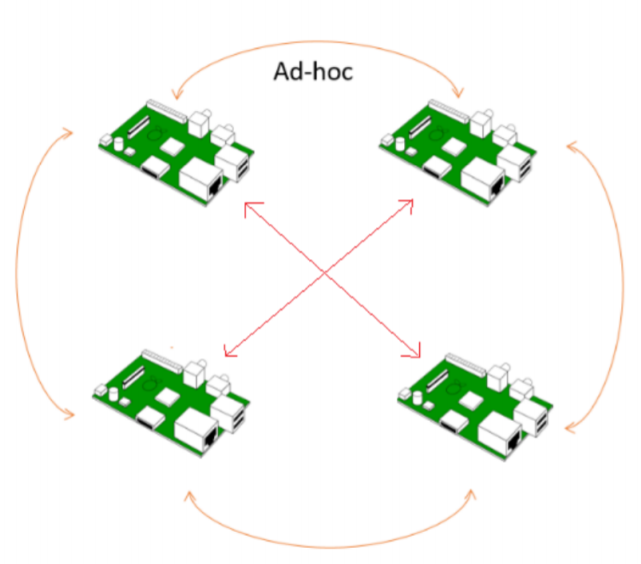
\includegraphics[width=0.4\textwidth]{Figuras/ad-hoc.PNG}   
	\caption{Exemplo de rede Ad Hoc.}
	\label{fig:figura1}
\end{figure}

\paragraph{} Atualmente a concepção de rede Ad Hoc é bastante utilizada, e se faz presente em diversas tecnologias de grande importância no dia a dia das pessoas. Um grande exemplo de rede Ad Hoc é o \textit{Bluetooth}, onde são usados, por exemplo, para comunicação de PCs com impressoras, mouses e teclados sem fio. 

\section{Histórico}
\paragraph{} As primeiras aparições de redes Ad Hoc foram datadas de 1972 em um projeto chamado \textit{Packet Radio Network} (PRNET) pela Agência de Investigação de Projetos Avançados de Defesa (DARPA), dos Estados Unidos.

\paragraph{} Em 1983 a DARPA, expandindo o PRNET, lançou o programa SURAN (\textit{Survivable Adaptive Network}), que foi de grande importância no suporte de grandes redes e no desenvolvimento de protocolos de rede adaptáveis às variações no meio.

\paragraph{} Um terceiro grande projeto sobre redes Ad Hoc foi o GloMo (\textit{Global Mobile Information Systems}), que teve início em 1994. Mais uma vez foi feito pela DARPA, esse projeto teve como grande diferencial o uso do padrão IEEE 802.11, o Wi-fi. Apesar da DARPA liderar essa inovação, o conceito de redes Ad Hoc já havia se expandido para o meio civil nessa época.

\section{Das Vantagens e Desvantagens}
\paragraph{} Vantagens:

\begin{itemize}
   \item Não precisa de uma estrutura fixa:  Otimizando o tempo e o custo de montagem, além de aumentar a mobilidade.
   \item Não apresenta terminais críticos:  A rede não é afetada se algum dispositivo falhar.
   \item Escalabilidade:  Novos terminais podem ser facilmente adicionados na rede.
   \item Conectividade: Dois nós quaisquer, podem se comunicar diretamente, se um estiver ao alcance do outro. 
   
\end{itemize}
 
\paragraph{} Desvantagens:
 
\begin{itemize}
   \item Menor alcance em relação a outros tipos de rede.
   \item Roteamento: A mobilidade dos nós e a topologia contribuem para aumentar o grau de complexidade do algoritmo de roteamento da rede.
   \item Por ser uma rede sem fio, a rede Ad Hoc também tem taxas de erros mais elevadas e menor banda passante do que as redes cabeadas.
\end{itemize}

\section{Redes Mesh}
\paragraph{} Entre as topologias aplicadas em redes MANET, a mais usada é a rede \textit{mesh}, uma rede em que os nós se conectam diretamente, dinamicamente e de maneira não hierárquica. Essa rede, pode ser representada pela seguinte figura:

\begin{figure}[!ht]
	\centering
	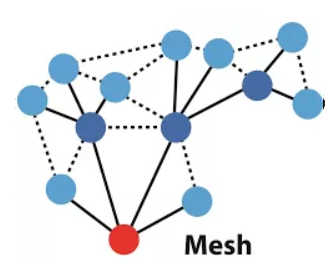
\includegraphics[width=0.4\textwidth]{Figuras/mesh.PNG}   
	\caption{Exemplo de rede \textit{mesh}. \citep{Mesh}}
	\label{fig:figura2}
\end{figure}

\paragraph{} Uma rede \textit{mesh} é caracterizada de duas formas, parcial e total. Na parcial nem todos os nós estão interconectados, já na forma total, ela apresenta todas as conexões possíveis. 

\paragraph{} Como essa rede dispõe de diversas conexões, para transmitir uma mensagem é preciso de técnicas de roteamento e algoritmos de auto-recuperação dos pacotes, em função dos diversos caminhos possíveis.
\chapter{IEEE 802.15.4}
\noindent

\section{Apresentação do protocolo}

\paragraph{}	O protocolo IEEE 802.15.4 é um padrão que define redes de área pessoal sem fio de baixas taxas (LR-WPAN), porém há implementações do protocolo que extravasam o limite de alcance de uma rede pessoal, assim podendo ser considerada como WAN. Ele especifica principalmente a camada física e a subcamada MAC, e pode operar com o IPv6.


\section{Escolha do IEEE 802.15.4}

\paragraph{}	Como o objetivo do projeto é fazer uma rede Ad Hoc com sistemas embarcados em VANTs, será muito importante que a rede ofereça recursos de escalabilidade, longa duração de bateria e confiabilidade. Requisitos encontrados no protocolo IEEE 802.15.4.

\paragraph{}	Além desses motivos, o IEEE 802.15.4 tem implementações comerciais de sucesso como o \textit{ZigBee}, que tem sido, constantemente, apresentado em diversos artigos acadêmicos \citep{CUNY} \citep{pfcmelhorqueonosso}- fatores que indicam a aplicabilidade desse protocolo.  

\section{Camadas do Modelo OSI no IEEE 802.15.4}
\subsection{Camada Física}
\paragraph{} A camada física (PHY) é responsável pela interface do meio de transmissão com a subcamada MAC. No protocolo IEEE 802.15.4 a camada física tem como funções principais a escolha de canais, sincronização de pacotes, modulação e demodulação. Além destas funções, a camada física provê mecanismos para passar e receber dados da subcamada MAC \citep{IEEE2016}. 

\subsubsection{Gerenciamento de Canais}
\paragraph{} O IEEE 802.15.4 trabalha em três bandas de frequências diferentes, centradas em 868 Mhz, 915 MHz e 2400 MHz. As bandas tem: 1, 10 e 16 canais respectivamente, conforme mostra a figura \ref{fig:figura3}.

\begin{figure}[!ht]
	\centering
	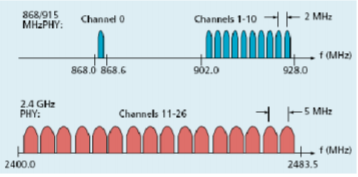
\includegraphics[width=0.5\textwidth]{Figuras/canais.PNG}   
	\caption{Canais do IEEE 802.15.4. \citep{Ufes}}
	\label{fig:figura3}
\end{figure}

\paragraph{} Para a escolha de canal, é feita uma varredura em uma determinada banda de frequência, permitindo que camadas superiores selecionem o canal apropriado. 

\paragraph{} O principal critério de escolha é pela detecção de energia, assim sendo, o canal de menor energia será o escolhido. Para isso o protocolo dispõe de um detector de energia que fornece, com um inteiro de 8 bits, o valor de potência do canal de até 10 dB acima da sensibilidade do receptor.

\paragraph{} A fim de eliminar interferências de outras redes, o IEEE 802.15.4 impõe um regime de rejeição de canais.

\paragraph{} Ao receber um sinal, o canal deve ser rejeitado,  caso haja um outro sinal do mesmo nível, ou mais fraco em um canal adjacente, ou ainda, um sinal de no máximo 24 dB mais forte em um canal alternado.

\subsubsection{Estrutura dos pacotes}

\paragraph{} Na camada física do IEEE 802.15.4,
 o pacote é dividido em 4 partes: preâmbulo, delimitador, cabeçalho e PHY \textit{Service Data Unit} (PSDU). Essa estrutura é representada pela figura \ref{fig:figura4}:
 
 \begin{figure}[!ht]
	\centering
	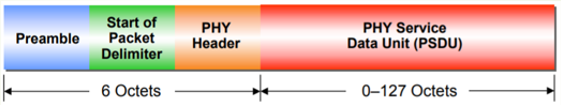
\includegraphics[width=0.5\textwidth]{Figuras/pacote_PHY.PNG}   
	\caption{Modelo de pacote da camada física. \citep{EATON}}
	\label{fig:figura4}
\end{figure}

 
 \paragraph{} O preâmbulo é constituído de 4 bytes que tem como principal função o treinamento do equalizador. A modulação que está sendo usada na transmissão será indicada por uma sequência de bits. No caso deste projeto, o padrão de cada byte será "01010101", que caracteriza o GFSK.
 
 \paragraph{} O delimitador (\textit{Start of Packet Delimeter}) são 8 bits pré-estabelecidos para indicar o final do preâmbulo e atua como um sincronizador. Para o IEEE 802.15.4 essa sequência será "11100101".
 
 \paragraph{} Cabeçalho PHY (PHR) é definido por apenas por 1 byte. Esse byte é constituído por 7 bits para definir o tamanho da PSDU e o oitavo bit é reservado.
 
 \paragraph{} O PSDU é o \textit{payload} da camada física e o seu tamanho pode variar de 0 à 127 bytes.
 
 \subsubsection{Parâmetros para o projeto}
 \paragraph{} O padrão IEEE 802.15.4 para a modulação GFSK utiliza os seguintes parâmetros (tabela \ref{tab:tabela1}):
 
\begin{table}[ht]
\centering
\caption{Parâmetros do IEEE 802.15.4 usados no projeto.}
\vspace{0.5cm}
\begin{tabular}{r|lr}
 
Modulação & GFSK \\
\hline
Banda de operação & 920 MHz \\
Taxa de bits & 100 kbps (100 kbauds) \\
Tamanho do canal & 2 Mhz \\
Potência de transmissão & Pelo menos -3 dBm \\
Sensibilidade do receptor & -85 dBm \\
Número de canais & 10 \\
Largura de banda & 2000 KHz 
 
\end{tabular}
\label{tab:tabela1}
\end{table}
 
\subsubsection{Modulação}
\paragraph{} O protocolo IEEE 802.15.4 permite o uso de diversas modulações, porém a modulação utilizada pelo rádio nRF24l01+ é a GFSK (\textit{Gaussian frequency-shift keying}).

\paragraph{} Essa modulação consiste no chaveamento deslocado de frequência binário com um filtro gaussiano na entrada do sistema. A consequência desse processo é a filtragem dos pulsos de dados para tornar as transições mais suaves. Sua principal vantagem é a redução da potência da banda lateral, assim reduzindo a interferência entre canais vizinhos. O protocolo utiliza um filtro cujo BT é de 0,5 e o índice de modulação do sinal é unitário.

\begin{figure}[!ht]
    \centering
    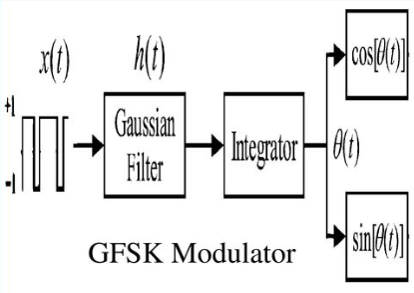
\includegraphics[width=0.4\textwidth]{Figuras/GFSK1.PNG}
    \caption{Diagrama de blocos da modulação GFSK. \citep{IEEE2015}}
    \label{fig:figura5}
\end{figure}
    
\begin{figure}[!ht]
    \centering
    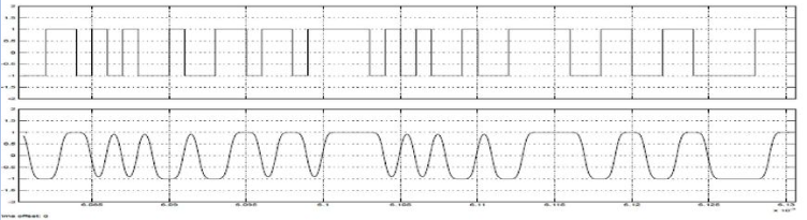
\includegraphics[width=0.6\textwidth]{Figuras/GFSK2.PNG}
    \caption{Comparação das modulações GFSK e FSK. \citep{IEEE2015}}
    \label{fig:figura6}
\end{figure}

\paragraph{} Para melhor funcionamento da modulação, o protocolo faz uso obrigatório \textit{Data Whitening}. Esse processo se fundamenta na descorrelação entre os bits a serem enviados, visando evitar sequências longas de bits iguais. 
 
\paragraph{} O \textit{Data Whitening} é o resultado do "ou exclusivo" entre os bits de entrada com pseudo-ruído de 9 bits gerado pelo mecanismo da figura \ref{fig:figura7}: 

\begin{figure}[!ht]
	\centering
	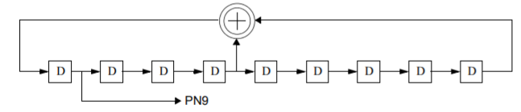
\includegraphics[width=0.5\textwidth]{Figuras/PN9.PNG}   
	\caption{Mecanismo de pseudo ruído de 9 bits. \citep{IEEE2015}}
	\label{fig:figura7}
\end{figure}

\paragraph{} Onde PN9 é a sequência definida pelo algoritmo da figura, com semente “111111111”.


\subsection{Subcamada MAC}
\paragraph{} A subcamada MAC é a parte inferior da camada de enlace, que fornece acesso às camadas superiores.

\paragraph{} Entre as suas principais funcionalidades estão a associação e desassociação de dispositivos na rede e o controle de acesso a canais associados. 

\paragraph{}Além dessas funções, a subcamada MAC é responsável por gerar \textit{beacons} de rede que permitem que os dispositivos localizem uma rede existente ou, no caso de redes TDMA, que forneçam uma indicação de tempo para os dispositivos clientes acessarem o canal durante períodos baseados em contenção e sem contenção.

\paragraph{} Para as camadas superiores, a subcamada MAC também oferece serviços de encaminhamento de dados destinados ou oriundos das camadas superiores (MCPS), e de mecanismo para controlar as configurações de comunicação, de rádio e funcionalidade de rede, da camada acima (MLME)\citep{IEEE2016}.

%\subsubsection{Channel Hopping}
%\paragraph{} Channel Hopping pelo dicionário da IEEE Standards significa alternar periodicamente o canal usando uma sequência conhecida tanto para envio como para recebimento dispositivos onde o quadro inteiro é enviado em um único canal. 

%\paragraph{} Os dispositivos podem saltar 

\subsubsection{Operação com \textit{Beacon}}
\paragraph{} Toda rede IEEE 802.15.4 usa \textit{beacons} de um coordenador ao unir dispositivos à rede. Nessa operação, o coordenador envia uma sequência de sinais de \textit{beacon}, contendo informações, que permitem que os nós da rede sincronizem suas comunicações. 

\paragraph{} Dois \textit{beacons} consecutivos costumam marcar o início e o fim de um superquadro. Um superquadro é uma estrutura de 16 intervalos de tempo que podem ser usados para comunicação.

\paragraph{} Um superquadro pode ser dividido em duas partes: Uma é a parte inativa que permite o coordenador entrar em modo de baixa potência; a outra, é a parte ativa que apresenta dois períodos principais o CAP (\textit{Contention access period}) e o CFP (\textit{Contention free period}). Conforme mostra a figura \ref{fig:figura8}:

\begin{figure}[!ht]
	\centering
	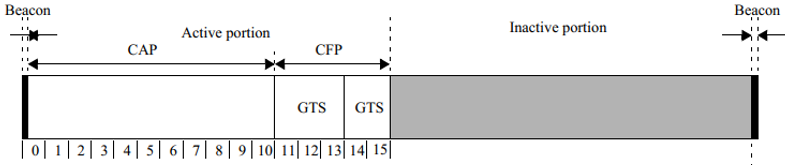
\includegraphics[width=0.6\textwidth]{Figuras/superquadro.PNG}   
	\caption{Estrutura de um Superquadro. \citep{IEEE2015}}
	\label{fig:figura8}
\end{figure}

\paragraph{} Durante o CAP, todos os quadros, com exceção dos quadros de ACK, usarão o mecanismo do CSMA/CA (descrito no tópico 3.3.2.2) para acessar o canal. Entre duas transmissões de quadro no CAP, a subcamada MAC exige um período entre quadros (IFS) para poder processar o último quadro enviado. 

\paragraph{} Ao contrário do CAP, as transmissões feitas dentro do CFP não utilizam CSMA/CA. Além disso, dentro do CFP ocorrem os GTS (\textit{Guaranteed Time Slot}), que são \textit{slots} do superquadro dedicados à comunicação entre um dispositivo e o coordenador da PAN. No superquadro podem haver até 7 GTSs.

\subsubsection{CSMA/CA}
\paragraph{} O CSMA/CA (Acesso múltiplo com verificação de portadora com prevenção de colisão) é um método de acesso múltiplo no qual a portadora, antes de iniciar a transmissão, escuta o canal e envia os dados, se esse estiver inativo; porém, se o canal estiver ocupado, a portadora aguardará, por um tempo aleatório, para a retransmissão.

\paragraph{} Para evitar o problema do terminal oculto, o CSMA/CA utiliza-se de pequenos pacotes chamados RTS (\textit{Ready to send}) e CTS (\textit{Clear to send}). O RTS é o pedido do terminal para poder realizar a transmissão, porém, só poderá enviar os pacotes após receber do ponto de acesso o CTS. Esse processo é eficiente pelo ponto de vista de que só poderá haver um CTS enquanto o canal estiver desocupado, porém essa prática pode congestionar o canal, se for utilizada em excesso \citep{Tanenbaum}.  

\paragraph{} Por conta de diversos terminais poderem ver o ponto de acesso e, pela dificuldade de se ouvir outras transmissões na rede, devido a longas distâncias, o método do CSMA/CA se tornou ideal para a rede ad hoc sem fio, que foi proposta, para este projeto.

\paragraph{} O IEEE 802.15.4 oferece diversos algoritmos de acesso randômico, porém o escolhido para o projeto foi o CSMA/CA com o fluxograma, conforme a figura \ref{fig:figura9}, onde "sucesso" representa a permissão para começar a transmissão, conforme a figura 3.7:

\begin{figure}[!ht]
	\centering
	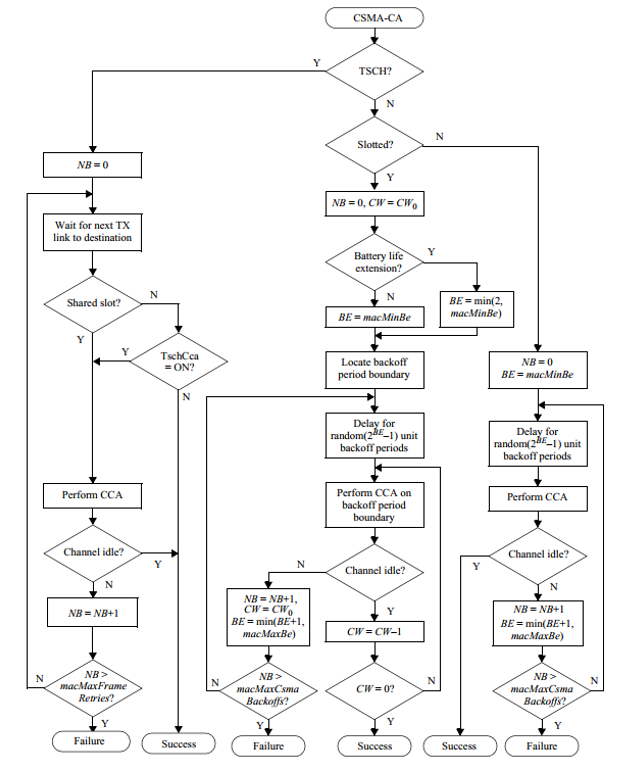
\includegraphics[width=0.6\textwidth]{Figuras/fluxograma_CSMA.PNG}   
	\caption{Fluxograma CSMA/CA do IEEE 802.15.4. \citep{IEEE2015}}
	\label{fig:figura9}
\end{figure}


\newpage
\subsubsection{Estrutura dos Pacotes}
\paragraph{} O pacote da subcamada MAC se encontra dentro da PSDU e é subdividida em três partes principais: MAC \textit{header} (MHR), MAC \textit{payload} e MAC \textit{footer} (MFR). Conforme mostram as figuras \ref{fig:figura10} e \ref{fig:figura11}:


\begin{figure}[!ht]
    \centering
    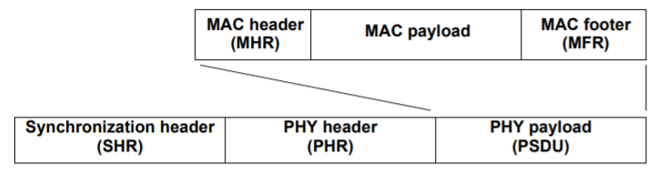
\includegraphics[width=0.6\textwidth]{Figuras/MAC1.PNG}
    \caption{Pacote MAC em relação à camada física. \citep{IEEE2015}}
    \label{fig:figura10}
\end{figure}
    
\begin{figure}[!ht]
    \centering
    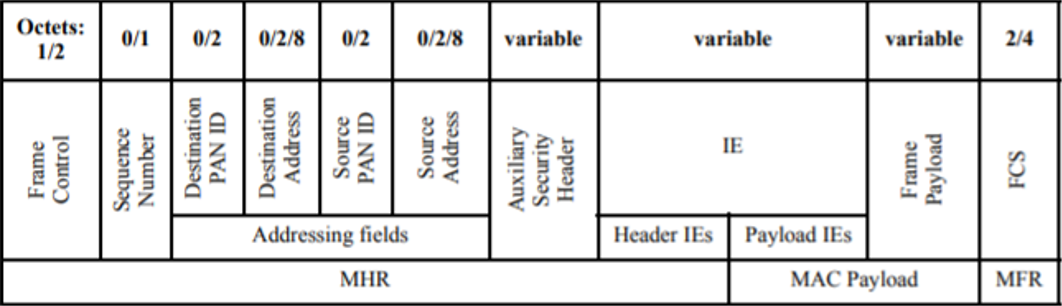
\includegraphics[width=0.6\textwidth]{Figuras/MAC2.PNG}
    \caption{Divisão do pacote da subcamada MAC. \citep{IEEE2015}}
    \label{fig:figura11}
\end{figure}

\paragraph{}A primeira parte do MHR é o \textit{Frame Control}, que é responsável por diversas configurações da transmissão. Uma dessas configurações é a definição do tipo do pacote. São usados os 3 primeiros bits para dizer se o pacote é um \textit{beacon}, se é de dados, de \textit{acknowledgment}, entre outros. O bit seguinte é o de habilitação de segurança, o qual não será habilitado para o projeto. Depois, vem o bit de pendência, que é enviado pelo dispositivo, caso tenha mais dados do que um único pacote permite. A seguir vem o AR (\textit{ACK request}) que especifica se é necessário um quadro de confirmação do receptor. O sétimo bit do \textit{Frame Control} é o de compressão do PAN ID. O oitavo e nono bits são respectivamente os indicativos de supressão do número de sequência e de presença do IE (\textit{Information Element}), ambos serão ausentes no pacote gerado para o projeto. Os dois bits do \textit{Destination Addressing Mode} e do \textit{Sorce Addressing Mode} serão "10" para endereços de 16 bits e "11" para endereços de 64 bits. Por fim, o \textit{Frame Control} especifica a versão do protocolo IEEE 802.15.4 que será usada no quadro sendo: "00" para a versão de 2003, "01" para a de 2006 e "10" para a atual. O \textit{Frame Control} pode ser melhor visualizado pela figura \ref{fig:figura12}: 

\begin{figure}[!ht]
	\centering
	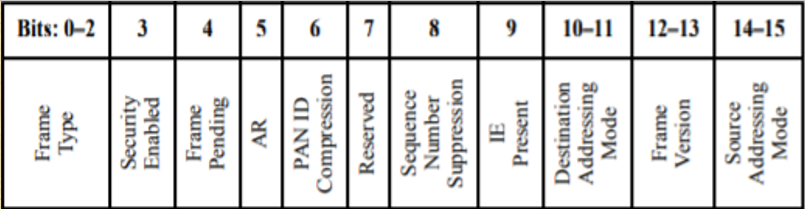
\includegraphics[width=0.6\textwidth]{Figuras/frame_control.PNG}   
	\caption{Divisão do campo \textit{Frame Control}. \citep{IEEE2015}}
	\label{fig:figura12}
\end{figure}

\paragraph{} Os campos de PAN ID, do destino e da fonte, apresentam um tamanho de 2 bytes, enquanto os endereços podem variar entre curtos (2 bytes) ou longos (8 bytes), de acordo com o especificado no \textit{Frame Control}.   

\paragraph{} As demais subdivisões do MHR, como o Número de sequência, o Cabeçalho de Segurança Auxiliar e o Elemento de Informação serão suprimidas no pacote do projeto, portanto, não serão abordados neste texto.

\paragraph{} O MAC \textit{Payload} será constituído por dados de informação e seu tamanho é variável de acordo com o tamanho do PSDU especificado na camada física.

\paragraph{} O MAC \textit{footer} contém CRC de 16 ITU-T e 32 bits equivalente ao ANSI X3.66-1979, e é formado pelo polinômio binário correspondente ao resto da divisão da sequência de bits do MHR e MAC \textit{payload} pelo polinômio gerador.

\paragraph{} Como o rádio nrf24l01+ permite no máximo de 16 bits de CRC, o polinômio gerador usado no projeto será de acordo com a seguinte forma:

\begin{equation}
    G_{16}(x) = x^{16} + x^{12} + x^5 + 1 
\end{equation}

\subsubsection{Rejeição de Pacotes}
\paragraph{} A subcamada MAC é capaz de filtrar os quadros recebidos de forma que só restem os quadros que são de interesse para a camada superior.

\paragraph{} O primeiro nível de filtragem ocorre quando os valores do MAC \textit{footer} estiverem incorretos. Como esse campo é de verificação de erros, qualquer pacote que tiver erro não será passado para a camada superior.

\paragraph{} O próximo nível de filtragem dependerá se o MAC estiver em modo promíscuo, neste caso, o pacote não receberá nenhum filtro após a primeira filtragem. Se não tiver em modo promíscuo, a próxima análise consiste em verificar se a subcamada está operando em varredura. Durante uma varredura, a subcamada MAC deve descartar todos os quadros recebidos pelo serviço de dados PHY.

\paragraph{} Por fim, será filtrado todo quadro que não contiver um tipo ou versão do protocolo. 

\subsubsection{6LoWPAN}
\paragraph{} O padrão IEEE 802.15.4 utiliza o IPv6 como protocolo de endereçamento, porém o IPv6 tem um tamanho de pacote maior que os 128 bytes disponíveis no PSDU. Para resolver esse problema, foi criado o 6LoWPAN (\textit{IPv6 in Low-Power Wireless Personal Area Networks Groups})\citep{6lowpan}.

\paragraph{} O 6LoWPAN foi uma solução da IETF para a adaptação do pacote IPv6 ao IEEE 802.15.4. Essa compressão de pacote permite dispositivos com baixo poder computacional usar a mais nova versão do protocolo IP. Para a realização da compressão, o 6LoWPAN utiliza de informações de protocolos de outras camadas.   

\paragraph{}Essa seção é baseada no padrão escrito pela IEEE-SA Standart Board \citep{IEEE2015}

\section{\textit{OpenThread}}
\subsection{O que é \textit{OpenThread}}
\paragraph{} \textit{OpenThread} é uma implementação do código do protocolo de rede \textit{Thread} feito pela Nest (uma empresa do grupo Google). A Nest trabalha na área de tecnologia para automação de serviços domésticos como termostatos via wi-fi, detectores de fumaça e sistemas de segurança programáveis. Para o funcionamento desses produtos, foi necessário o uso do protocolo \textit{Thread}, que é uma tecnologia de rede \textit{mesh} de baixo consumo, baseada em IPv6 \citep{Open}. 

\paragraph{} O \textit{OpenThread} implementa as camadas de rede \textit{Thread} como a do IEEE 802.15.4, e tem como principais recursos a segurança, com autenticação dos dispositivos de rede e criptografia das comunicações, confiabilidade, eficiência em relação ao consumo de energia e escalabilidade da rede. O \textit{OpenThread} trabalha com a versão de 2006 do IEEE 802.15.4. 

\subsection{Funções do \textit{Openthread}}
\paragraph{} Na rede \textit{Thread} existem duas funções de encaminhamento: o roteador e o dispositivo final (ED). Conforme mostra a figura \ref{fig:figura13}:

\begin{figure}[!ht]
	\centering
	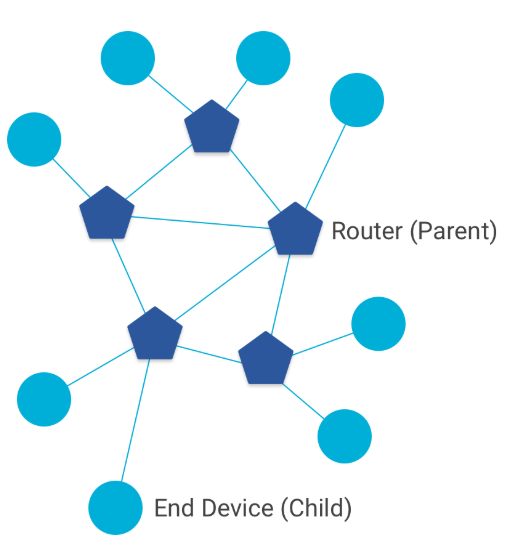
\includegraphics[width=0.4\textwidth]{Figuras/openthread.PNG}   
	\caption{Exemplo de rede Thread. \citep{Open}}
	\label{fig:figura13}
\end{figure}

\paragraph{}O roteador é um nó que encaminha pacotes para os dispositivos da rede, além de introduzir de forma segura novos dispositivos nela. Já o dispositivo final, não encaminha pacotes para outros dispositivos de rede, pois se comunica, principalmente, com um único roteador.
O protocolo \textit{Thread} nomeia a relação do roteador com o dispositivo final de relacionamento pai-filho, onde o roteador é o pai e o ED é o filho.

\paragraph{} Numa rede, pode acontecer de um roteador não ter filhos, então ele pode ser rebaixado e operar como um dispositivo final. O mesmo pode acontecer com um ED que ao ser o único nó ao alcance de um novo dispositivo que deseja ingressar na rede, ele pode operar como um roteador.

\paragraph{} Na rede \textit{Thread} existem também o \textit{Thread} Líder e o Roteador de borda. O \textit{Thread} Líder é o roteador responsável por gerenciar o conjunto de roteadores na rede, ele é dinamicamente auto-eleito e distribui informações de configuração em toda a rede. O Roteador de borda é um dispositivo que pode encaminhar informações para uma rede externa não \textit{Thread}.

\paragraph{} A rede \textit{Thread} permite apenas um líder, 32 roteadores e 511 dispositivos finais, por roteador.

\subsection{Endereçamento IPv6}
\paragraph{} Para fazer o endereçamento, primeiramente o \textit{Thread} gera um localizador de roteamento (RLOC). Esse localizador é gerado de forma que cada roteador mantenha uma tabela de todos os seus filhos, cuja combinação (ID do roteador + 0 + ID do filho) identifica de forma exclusiva um dispositivo dentro da topologia, então cada dispositivo terá um RLOC diferente. Como todos os dispositivos recebem uma ID, o RLOC de 16 bits gerado, quando os IDs do roteador e do filho forem iguais a 1, será segundo a figura \ref{fig:figura14}. O RLOC de 16 bits do roteador será gerado da mesma forma, só que o ID do filho será igual a zero;

\begin{figure}[!ht]
	\centering
	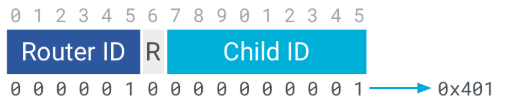
\includegraphics[width=0.5\textwidth]{Figuras/RLOC16.PNG}   
	\caption{Exemplo de localizador de roteamento de 16 bits. \citep{Open}}
	\label{fig:figura14}
\end{figure}

\paragraph{} Esse localizador de roteamento, faz parte do identificador de interface (IID), que corresponde aos últimos 64 bits do endereço IPv6. Então o IID é sempre do tipo 0000:00ff:fe00:RLOC16.

\paragraph{} Por fim, o RLOC completo será a combinação do prefixo local de malha com o IID. Dessa forma, o RLOC representa um dos tipos de endereço \textit{unicast} IPv6 que um dispositivo \textit{Thread} pode ter.

\subsection{Criação de Redes}
\paragraph{} Para que um dispositivo se junte a uma rede ou crie uma rede própria, é preciso que ele transmita um \textit{Beacon request}, em um canal específico para todo seu alcance. Um outro dispositivo, ao receber essa solicitação, responde com um \textit{beacon} que contém seu PAN ID, XPAN ID, bem como o Nome da Rede. Esse processo é realizado para todos os canais, assim podendo se conectar a uma rede ou criar uma rede própria.

\paragraph{} O \textit{Mesh Link Establishment} (MLE) é o protocolo que vai configurar os enlaces e disseminar as informações sobre a rede. Esse protocolo fornece informações do tipo: Dados do líder, dados de rede e propagação das rotas.

\paragraph{}Para criar uma nova rede, um dispositivo terá que selecionar o canal menos ocupado, além de um PAN ID que não esteja em uso. Após esse processo, ele se declarará líder e envia mensagens de informações MLE para os outros dispositivos 802.15.4.

\subsection{Seleção de Roteador} 
\paragraph{} Conjunto Dominante Conectado é um sistema que garante um nível mínimo de redundância para a rede. Para isso, tem que haver apenas um caminho de roteadores entre dois roteadores. Todos os roteadores poderão se comunicar, e cada dispositivo final deverá estar conectado diretamente a um roteador.

\paragraph{} O número de roteadores em uma rede \textit{Thread} é variável, de acordo com as suas necessidades. Roteadores devem ser adicionados, para aumentar a cobertura, aumentar a diversidade de caminhos, manter redundância e conectar mais dispositivos finais. A remoção se faz necessária, para reduzir o estado de roteamento, e permitir novos roteadores em outras redes. 

\chapter{RNDIS}
\noindent

\paragraph{} A Especificação da Interface de \textit{Driver} de Rede Remota (RNDIS) é um protocolo da \textit{Microsoft} que atua principalmente sobre o USB, e fornece um link \textit{Ethernet} virtual para os sistemas operacionais \citep{RNDIS}.

\section{USB}

\paragraph{} 
Nesta seção iremos ver alguns conceitos do protocolo USB que serão necessários para posterior entendimento do sistema desenvolvido, que foram aplicados na implementação do código desenvolvido no projeto. Como base para implementação foi utilizado as bibliotecas padrão do fabricante do microcontrolador e uma biblioteca utilizada pela IMBEL, que é restrita para uso comercial. E para a depuração foi utilizado o software USBLyzer e uma documentação de assistência a implementações práticas, descrita por uma fabricante de dispositivos IOT. 

USB (\textit{Universal Serial Bus}) é uma interface para conexão de dispositivos, mais conhecida de todos os tempos, foi desenvolvida em 1996 e popularizada nos anos 2000. No decorrer do tempo a USB passou por três significativas revisões, estando atualmente na versão 3.0, que suporta transmissão de vídeo com resolução \textit{full} HD em tempo real.

\subsection{\textit{Endpoint}}

\paragraph{}Um sistema USB é formado por um \textit{host} e múltiplos periféricos conectados através de um único canal. O \textit{host} atribui um endereço de 7 bits a cada periférico, de forma que um host pode estar ligado a até 127 dispositivos.

\paragraph{}A transmissão de dados pelo protocolo se faz através de \textit{buffers} endereçáveis, conhecidos como \textit{endpoints}, sendo que cada dispositivo possui múltiplos \textit{endpoints}, que são unidirecionais, tendo convencionada a direção de \textit{host} para periférico como OUT, e de periférico para \textit{host} como IN.

\paragraph{}Além de endereço e direção, cada \textit{endpoint} está relacionado a um tipo de transmissão. As transmissões de controle são usadas para pacotes de configuração, requisição e comando. As transmissões de \textit{interrupt} garantem a latência mínima para recepção dos pacotes.

\paragraph{}As transmissões do tipo \textit{bulk} são usadas para transmissão de pacotes grandes de dados, até 1500 bytes por pacote, sem garantia de velocidade e latência. Transmissões do tipo \textit{isochronous} são usadas para \textit{streaming} de vídeo e áudio em tempo real com largura de banda reservada, e sem checagem de erro.

\subsection{Descritores}

\paragraph{}Quando um periférico é conectado a um \textit{host}, aquele envia informações sobre suas funções para este; configurações do dispositivo, e configurações de cada \textit{endpoint}. Os dispositivos USB são ainda divididos em classes e subclasses pré-determinadas pelo USB fórum, para controlar a evolução e a padronização do protocolo.

\paragraph{}Um dispositivo de mouse USB, por exemplo, pertence a classe \textit{Humam Interface Device} (HID), e possui três \textit{endpoints}: Os \textit{endpoints} IN e OUT de controle e um \textit{endpoint interrupt} IN para envio de eventos relacionados ao usuário, como um clique de botão ou movimento do dispositivo.

\subsection{Interface e configuração}

\paragraph{}O protocolo USB especifica ainda que cada dispositivo pode ter múltiplas configurações e múltiplas interfaces, permitindo que o \textit{host} escolha a maneira como irá utilizar o dispositivo (através da escolha da configuração), e quais recursos do dispositivo irá utilizar (através da escolha das interfaces).

\subsection{Transações de controle}

Transações de controle são sempre iniciadas pelo \textit{host} com um pacote de 8 bytes de \textit{setup}, que identifica o tipo de pacote a direção e a função do mesmo. Em seguida os pacotes de dados e por fim um pacote de status indicando o estado do dispositivo ou do \textit{host} dependendo do tipo de transação.

No caso do protocolo do protocolo RNDIS é através do pacote de \textit{setup} que o \textit{host} configura o dispositivo e obtém as especificações do mesmo, como endereço físico do díspositivo, banda disponível, etc. O dispositivo e \textit{host} somente estão aptos a transmitir pacotes de dados com \textit{frames ethernet} após a fase de configurações. 

\subsection{Transações de \textit{interrupt}}

Essas transações determinam um tempo mínimo para serem notificadas, são ideias para notificar a ocorrência de eventos, e costumam ser utilizadas por dispositivos que trabalham sobre eventos como o mouse e o teclado, ou seja, dispositivos de interface humana.

No protocolo RNDIS é utilizado um \textit{endpoint} do tipo \textit{interrupt} para notificar o \textit{host} sobre mensagens a serem lidas no \textit{endpoint} de controle. É utilizado dessa forma para contornar a limitação do \textit{endpoint} de controle que aceita somente transações iniciadas pelo \textit{host}, tornando o canal de configuração em um canal \textit{full duplex}.

\subsection{Transações de \textit{bulk}}

São usadas para transmitir grandes blocos de dados, possuem mecanismo automático de verificação de erro e mecanismo de retransmissão. Esses mecanismos possuem maior latência, mas garantem a entrega dos dados, por isso são muito usados para transmissão de grandes blocos de dados, que podem ser fragmentados, sem que se precise implementar algorítmos de retransmissão.

No caso do RNDIS são usados para transmitir \textit{frames ethernet}, os \textit{frames} são fragmentados, em pacotes de 64 bytes e transmitidos pelo \textit{endpoint}. Se o tamanho do \textit{frame} for múltiplo de 64 bytes é enviado um pacote adicional, de forma que um pacote menor do que 64 bytes indique o fim de um \textit{frame ethernet}.

%Os pacotes USB são divididos em Token, data, handshake, special. Transações em %endpoints de controle são sempre iniciadas pelo host por um pacote de 
\chapter{Propagação de Ondas Usando o modelo de 2 Raios}
\noindent

\section{Propagação de Ondas Eletromagnéticas no RF}
\paragraph{}À medida em que os sistemas de comunicação sem fio se tornam mais presentes nas diversas aplicações de telecomunicações, uma compreensão a cerca da propagação de ondas na faixa RF (\textit{Radio Frequency}) se torna cada vez mais importante. A modelagem da propagação das ondas nessa faixa, 1 MHz a 300 GHz, ainda é um campo de estudos em crescimento, um fato que é caracterizado pelos diversos modelos existentes, bem como pelo surgimento de novos. No espaço livre, as ondas eletromagnéticas são modeladas como saindo da fonte em todas as direções, resultando numa frente de onda esférica. À medida em que a onda se afasta da fonte, a sua frente de onda converge para uma frente plana, pois é dessa forma que ela é utilizada nos modelos de propagação.

\paragraph{}As ondas RF apresentam três modos de propagação: Onda terrestre, onda direta e onda celeste. Para a faixa UHF (\textit{Ultra High Frequency}), será analisada somente o da onda direta, sendo os outros modos pouco relevantes para essa faixa de frequência. Sistemas UHF podem empregar antenas de tamanho moderado, que por sua vez, podem se tornar uma boa escolha para sistemas móveis. Algumas das aplicações para esses sistemas incluem rádio FM, telefones celulares, GPS (\textit{Global Positioning System}) e comunicação de rádio em aeronaves.




\paragraph{}O objetivo de modelar a propagação das ondas é simular o funcionamento de um sistema de comunicações de forma que se saiba se ele atenderá, ou não aos requisitos estabelecidos para ele. 

\paragraph{}A gama de modelos teóricos é extensa, sendo que o modelo teórico escolhido deve ser de acordo com o meio pelo qual as ondas se propagam. O que será utilizado no presente trabalho é o modelo de 2 raios, porque ele permite analisar como as  características do meio, da altura de voo dos VANT's, bem como da distância entre eles podem influenciar na potência recebida pela antena do VANT receptor. 

\section{Regiões de Campo}

\paragraph{}O espaço que envolve uma antena é usualmente subdividido em três regiões: reativa de campo próximo, campo próximo radiante, e campo distante. Essas regiões são designadas para identificar a estrutura de campo em cada uma. Embora  não haja nenhuma mudança abrupta nas configurações do campo quando este atravessa a fronteira que subdivide essas regiões, existem diferenças bem específicas entre elas.

\paragraph{}A região de campo próximo reativo é definido como a região que imediatamente envolve a antena, onde o campo reativo predomina. Para a maioria das antenas, essa é a região que existe para $R < 0.62sqrt(\frac{D^3}{\lambda})$ \citep{balanis} da superfície da antena, onde $\lambda$ é o comprimento de onda de operação e D é a maior dimensão da antena.

\paragraph{}O campo próximo radiante, também conhecido como região de Fresnel, é definido como a região do campo de uma antena entre o campo próximo reativo e o campo distante. Nessa região, predomina o campo radiante, sendo que a distribuição angular do campo depende da distância da região até a antena. Caso a máxima dimensão da antena seja pequena em relação ao comprimento de onda, essa região não deve existir. No entanto, se o maior comprimento da antena é grande comparado ao comprimento de onda, a região de campo próximo radiante deve ser definida por $0.62\sqrt(\frac{D^3}{\lambda})\leq R \leq 2\frac{D^2}{\lambda}$ \citep{balanis}.

\paragraph{}A região de campo distante é definida como a região do campo de uma antena onde a distribuição angular do campo é essencialmente independente da distância para a antena. Se a antena apresenta uma máxima dimensão D, o campo distante, ou a região de \textit{Fraunhofer}, é a região distante de R da antena tal que $R \geq 2\frac{D^2}{\lambda}$ \citep{balanis}. Nessa região, as componentes dos campos são essencialmente transversais, sendo a frente de onda uma frente de onda plana.

\section{Efeitos da Curvatura da Terra}

\subsection{Refração Atmosférica}

\paragraph{}A mudança gradual no índice de refração com a altura, faz com que a trajetória das ondas eletromagnéticas, que estão se propagando na troposfera, sofra uma determinada inclinação. Se a atmosfera fosse homogênea, a onda seguiria uma trajetória retilínea e o horizonte físico coincidiria com o horizonte RF. Essa característica do meio faz com que ocorra um aumento na distância aparente do horizonte, conforme mostra a figura a seguir:

\FloatBarrier
\begin{figure}[!htp]
\centering
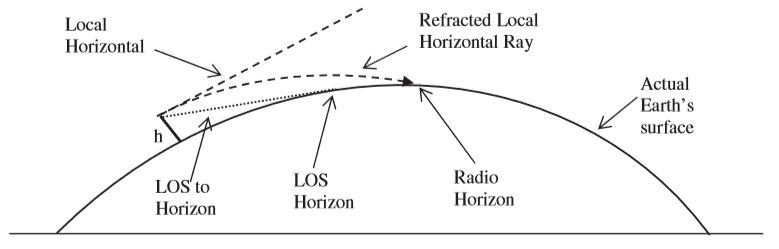
\includegraphics[scale = 0.5]{Figuras/refracao.JPG}
\caption{Efeito da troposfera na direção de propagação da EM, \citep{seybold}}
\end{figure}
\FloatBarrier

\paragraph{}Para facilitar os cálculos na modelagem, convém que se utilize o modelo de Terra Equivalente, pois ele permite que a modelagem seja feita considerando uma trajetória retilínea para os raios. Na modelagem utilizada, a terra possuirá um raio equivalente, tal:

\begin{equation}
    R_T^{eq} = KR_T
    \label{1}
\end{equation}

\paragraph{}Onde $R_T$ é o raio da terra, $R_T^{eq}$ é o raio equivalente da terra e K é o fator de raio equivalente da terra, onde $K = \frac{4}{3}$ para a atmosfera padrão. Assim, temos o seguinte cenário:

\FloatBarrier
\begin{figure}[!htp]
\centering
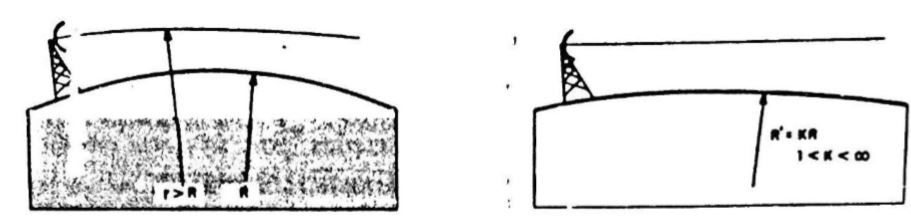
\includegraphics[scale = 0.5]{Figuras/Mod_Terr_Equ.JPG}
\caption{Modelo de Terra Equivalente \citep{Andrezo}}
\end{figure}
\FloatBarrier

\subsection{Distância de Horizonte e Distância do Limiar de Visada}

\paragraph{}Veja a seguinte figura:

\FloatBarrier
\begin{figure}[!htp]
\centering
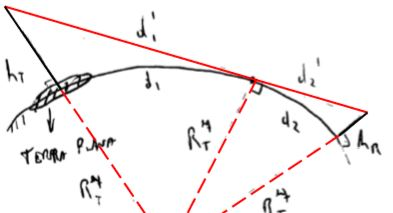
\includegraphics[scale = 0.5]{Figuras/Dist_Hor.JPG}
\caption{Modelo de Terra Equivalente \citep{Andrezo}}
\end{figure}
\FloatBarrier


\paragraph{}Quando $h_T << d_1$ e $h_R << d_2$, então $d1 \approx d'_1$ e $d_2 \approx d'_2$. Assim:

\begin{equation}
    d_1 = d'_1
    \label{2}
\end{equation}

\begin{equation}
    d_1^2 =  (h_T + R_T^{eq})^2 - R_T^{eq2}
    \label{3}
\end{equation}

\begin{equation}    
    d_1 = \sqrt{h_T^2 + 2h_TR_T^{eq}}
    \label{4}
\end{equation}

\paragraph{}Como $h_T << R_T^{eq}$:

\begin{equation}
    d_1 = \sqrt{2h_TR_T^{eq}}
    \label{5}
\end{equation}

\paragraph{}$d_1$ é a distância de horizonte da antena transmissora.

\paragraph{}Analogamente:

\begin{equation}
    d_2 = \sqrt{2h_RR_T^{eq}}
    \label{6}
\end{equation}

\paragraph{}Assim, a distância de visada $d_h$ é definida por:

\begin{equation}
    d_h = d_1 + d_2
    \label{7}
\end{equation}

\begin{equation}
    d_h = \sqrt{2R_T^{eq}}(\sqrt{h_T} + \sqrt{h_R})
    \label{8}
\end{equation}

\paragraph{}Na prática, é aceitável a aproximação de Terra plana ao longo de todo o trecho menor que a distância de horizonte, para cenários sem obstruções. Quando a distância entre as antenas é maior do que a distância de horizonte, se utiliza o modelo de 2 raios para terra esférica \citep{Andrezo}.



\section{Parâmetros fundamentais da Antena}

\subsection{Introdução}Uma antena é definida pelo \textit{IEEE Standard Definitions of Terms for Antennas} como um meio para radiar ou receber ondas rádio. Em outras palavras, a antena é uma estrutura tradicional entre o espaço livre e um dispositivo de guiamento \citep{balanis}. Para descrever o desempenho de uma antena, definições de vários parâmetros são necessários. Dentre eles, os principais que foram utilizados nesse projeto são: a diretividade e o ganho da antena.

\subsection{Diretividade}A diretividade de uma antena $D$ é definida como a razão da intensidade de radiação $U$ numa dada direção da antena com a intensidade de radiação média em todas as direções $U_0$. A intensidade de radiação média é igual a potência total radiada $P_{rad}$ pela antena dividida por 4$\pi$ \citep{balanis}. De forma mais simples, a diretividade  de uma fonte anisotrópica é igual a razão entre sua intensidade de radiação numa dada direção e a intensidade de radiação de uma fonte isotrópica.

\begin{equation}
    D = \frac{U}{U_0}
    \label{9}
\end{equation}

Onde:

\begin{equation}
    U_0 = \frac{P_{rad}}{4\pi}
    \label{10}
\end{equation}

\paragraph{}Portanto:

\begin{equation}
    D = 4\pi\frac{U}{P_{rad}}
    \label{32}
\end{equation}

\paragraph{}A direção de máxima intensidade de radiação (\textit{Diretividade Máxima}) é expressa como:

\begin{equation}
    D_{max} = D_0
    \label{33}
\end{equation}

\begin{equation}
    D_{0} = \frac{4\pi U_{max}}{P_{rad}}
    \label{34}
\end{equation}

\subsection{Ganho}

\paragraph{}Outra medida eficiente que descreve o desempenho da antena é o seu \textit{ganho}. Embora o ganho da antena esteja diretamente relacionado à diretividade, é uma medida que leva em consideração tanto a eficiência da antena como suas capacidades direcionais.

\paragraph{}O ganho de uma antena numa dada direção $G(\theta, \phi)$ é definido pela razão da intensidade numa dada direção $U(\theta, \phi)$, com a intensidade de radiação que seria obtida se a potência aceita pela antena fosse radiada isotropicamente \citep{balanis}. A intensidade de radiação correspondente a potência radiada isotropicamente é igual a potência de entrada da antena $P_{in}$, dividida por $4\pi$.

\begin{equation}
    G(\theta, \phi) = 4\pi\frac{U(\theta,\phi)}{P_{in}}
    \label{35}
\end{equation}

\paragraph{}A potência radiada relaciona-se com a potência de entrada na antena através da seguinte relação:

\begin{equation}
    P_{rad} = e_{cd}P_{in}
    \label{36}
\end{equation}

\paragraph{}Onde $e_{cd}$ é a eficiência de radiação (adimensional).

\paragraph{}Substituindo $P_{in}$ da equação \ref{36}, na equação \ref{35}, temos que:

\begin{equation}
    G(\theta, \phi) = e_{cd}[4\pi\frac{U(\theta, \phi)}{P_{rad}}]
    \label{37}
\end{equation}

\paragraph{}Que está relacionado a diretividade por:

\begin{equation}
    G(\theta,\phi) = e_{cd}D(\theta,\phi)
    \label{39}
\end{equation}

\subsection{Dipolo de meia onda}

\paragraph{}A antena dipolo de meia onda é uma das mais utilizadas atualmente em várias aplicações, principalmente porque a sua resistência de radiação é 73 ohms, que é bem próxima dos 50-ohm ou 75-ohm das impedâncias características de algumas linhas de transmissão \citep{balanis}.

\paragraph{} A intensidade de radiação de um dipolo de meia onda, alimentada por uma corrente $I_0$ e impedância característica $\eta$, é dada por \citep{balanis}:


\begin{equation}
    U(\theta) = \eta \frac{|I_0|^2}{8\pi^2}\sin^3\theta
    \label{40}
\end{equation}

\paragraph{}E a sua potência de radiação é dada por:

\begin{equation}
    P_{rad} = \eta \frac{|I_0|^2}{8\pi}C_{in}(2/pi)
    \label{41}
\end{equation}

\paragraph{}
Onde $C_{2\pi} = 2.435$ \citep{balanis}.


\paragraph{}Substituindo as expressões \ref{41} e \ref{40}, em \ref{34}, temos que:

\begin{equation}
    D(\theta,\phi) \approx 1.643\sin^3 \theta
    \label{42}
\end{equation}

\begin{equation}
    D(\theta) \approx 1.643\sin^3 \theta
    \label{43}
\end{equation}



\paragraph{}Portanto, substituindo a expressão \ref{43} na expressão \ref{39}, temos :

\begin{equation}
\label{Ganho}
    G(\theta,\phi) = 1.643e_{cd}\sin^3\theta
\end{equation}

\section{Modelo de dois raios}

\FloatBarrier
\begin{figure}[!htp]
\centering
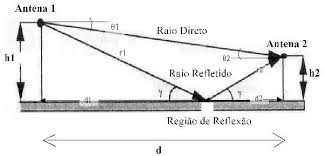
\includegraphics[scale = 0.8]{Figuras/images.jpg}
\caption{Modelo de 2 Raios Terra Plana}
\end{figure}
\FloatBarrier



\paragraph{}Nesse modelo, existem duas antenas, sendo uma transmissora de altura $h_t = h_1$ e uma receptora de altura $h_r = h_2$, separadas por uma distância d. O meio possui uma condutividade $\sigma$ e desvio-padrão das irregularidades de altura $\Delta h$. Nesse modelo, dado que a polarização da onda é perpendicular, o campo elétrico no receptor é expresso por:

\begin{equation}
\label{Mod2Raios}
    E = e^{-j\beta r_d}(E_{0d}F_{T}(\theta_i^{Tx})F_{R}(\theta_i^{Rx})+E_{0r}F_{T}(\theta_r^{Tx})F_{R}(\theta_r^{Rx})\rho_s\Gamma(\theta)e^{-j\beta\triangle r_d})
\end{equation}

\paragraph{}Sendo E o campo elétrico resultante da interferência entre o campo elétrico refletido no solo, e o campo elétrico que se propaga diretamente da antena transmissora. $E_{0d}$ e $E_{0r}$ são os campos elétricos que se propagam no ar livre, direto e refletido, respectivamente, dados por:

\begin{equation}
    {E_{Od}}^2 = \frac{30EIRP}{r_d^2}
\end{equation}

\begin{equation}
    {E_{Or}}^2 = \frac{30EIRP}{r_r^2}
\end{equation}

\paragraph{}Onde EIRP (\textit{Effective Isotropic Radiated Power}) é a potência efetivamente radiada. Ela é função da potência transmitida $P_t$:

\begin{equation}
    EIRP = P_tG_t
\end{equation}


\paragraph{}Na expressão \ref{Mod2Raios}, $F_x(\theta)$ é a função de radiação direcional da antena x, $\theta_i^{Tx}$ e $\theta_r^{Tx}$ são os ângulos de azimute com a direção da antena em relação a vertical e $\Delta r$ é a diferença de percurso entre o raio direto $r_d$ e o refletido $r_r$. 



\paragraph{} O coeficiente de reflexão $\Gamma(\theta)$ depende do meio no qual ocorre a propagação, e do ângulo de incidência da onda refletida $\theta_i$. A sua expressão depende também do tipo de polarização da onda:



\paragraph{}Para polarização perpendicular:

\begin{equation}
    \Gamma(\theta_i) = \frac{cos\theta_i - \sqrt{\frac{\epsilon_{1c}}{\epsilon_{2c}}}\sqrt{1 - \frac{\epsilon_{2c}}{\epsilon_{1c}}{sen\theta_i}^2}}{cos\theta_i + \sqrt{\frac{\epsilon_{1c}}{\epsilon_{2c}}}\sqrt{1 - \frac{\epsilon_{2c}}{\epsilon_{1c}}{sen\theta_i}^2}}
\end{equation}



\paragraph{}Para polarização horizontal:

\begin{equation}
    \Gamma(\theta_i) = \frac{-\cos\theta_i + \sqrt{\frac{\epsilon_{1c}}{\epsilon_{2c}}}\sqrt{1 - \frac{\epsilon_{1c}}{\epsilon_{2c}}{\sin\theta_i}^2}}{\cos\theta_i + \sqrt{\frac{\epsilon_{1c}}{\epsilon_{2c}}}\sqrt{1 - \frac{\epsilon_{1c}}{\epsilon_{2c}}{\sin\theta_i}^2}}
\end{equation}


\paragraph{}A relação do coeficiente de reflexão com o meio está expresso na permissividade complexa, que é dada por:

\begin{equation}
    \epsilon_c = \epsilon - j\frac{\sigma}{\omega}
\end{equation}

\paragraph{}Onde $\epsilon$ é a permissividade do meio, e $\omega = 2\pi f$, sendo f a frequência na qual a onda está se propagando.

\paragraph{}Por fim, deve-se levar em consideração a perda devido á rugosidade do solo. Para isso, é feita a análise do critério de Raylegh. Onde analisamos a diferença de fase entre as frentes de onda refletidas pela superfície $\triangle\phi$, sendo \citep{Andrezo}:

\begin{equation}
    \triangle\phi = \frac{4\pi\Delta hcos\theta_i}{\lambda}
\end{equation}

\paragraph{}Se $\triangle\phi < \frac{\pi}{2}$, conclui-se que a superfície é lisa, não havendo necessidade de levar em consideração a perda por rugosidade.

\paragraph{}Se $\triangle\phi > \frac{\pi}{2}$, a perda por rugosidade deverá ser levada em consideração, multiplicando-se o coeficiente de reflexão pelo fator de perda por espalhamento $\rho_s$:

\begin{equation}
    \rho_s = e^{-0.5{\Delta \phi}^2}
\end{equation}

\paragraph{}Dessa forma, ao se analisar a propagação das ondas eletromagnéticas num determinado meio, serão aferidos quais os efeitos, tanto do meio, caracterizados pela perda por propagação no espaço livre, reflexão no solo e pela rugosidade do mesmo, quanto das características da própria antena, tais como altura e polarização.

\paragraph{}No presente trabalho, será analisada para alguns cenários, a potência recebida pela antena receptora $P_r$. Calcularemos ela, utilizando a densidade de potência irradiada $S$ por uma antena no espaço livre:

\begin{equation}
    S = \frac{|E|^2}{120\pi}
\end{equation}

E a área efetiva da antena receptora $A_{em}$ \cite{balanis}:

\begin{equation}
    A_{ef} = \frac{\lambda^2G_r}{4\pi}
\end{equation}

\paragraph{}Finalmente:

\begin{equation}
    P_r = SA_{ef}
\end{equation}

\chapter{Codificação}
\section{BCH}

\paragraph{}O BCH é uma codificação do tipo cíclica, que tem por particularidade poder corrigir um certo número de erros em qualquer posição do código. BCH são as iniciais de Bose-Chaudhuri-Hocquenghem que corresponde aos sobrenomes dos inventores dessa codificação.

\paragraph{} Os códigos BCH são utilizados em diversas aplicações, tais como: comunicações por satélite, leitores de CDs , de DVDs e de códigos QR.

\paragraph{}O código BCH pode ser construído da seguinte maneira: Seja $m_i(x)$ um polinômio mínimo binário com coeficientes em GF(q) e $a^i$ é um elemento do GF(q), onde 'a' e 'i' são inteiros e 'q' é um número primo. Então existe um polinômio gerador formado segundo a equação \ref{eq1}:

\begin{equation}
\label{eq1}
G(x) = MMC(m_1(x),…, m_{(d - 1)}(x))
\end{equation}

\paragraph{} Onde d + 1 é igual ao q elevado ao comprimento do código. 

\paragraph{} Então, como todo código cíclico, a palavra código será $x^r.M(x) + R(x)$. Onde M(x) é a mensagem, r o grau do polinômio gerador e R(x) o resto da divisão de $x^r$.M(x) por G(x).

\paragraph{} A decodificação começa a partir do cálculo do vetor síndrome, que é a soma da palavra código com um vetor de erro desconhecido, se o vetor síndrome tiver algum valor diferente de zero, então haverá erros na palavra código. Através do algoritmo de Berlekamp-Massey \citep{berlekamp}, podemos achar o polinômio de localização do erro. Então, a partir desse polinômio é possível corrigir os erros da palavra código, já que suas raízes são as localizações dos erros. Por fim a mensagem é reconstruída pela divisão do código corrigido pelo polinômio gerador.

\section{Reed-Solomon}
\paragraph{} A codificação Reed-Solomon é um grupo de códigos de correção de erro. Um dos integrantes desse grupo é o próprio BCH, porém essa nova codificação é baseada na correção de símbolos. 

\paragraph{}Essa codificação além das tecnologias citadas no BCH, ela é utilizada em transmissões de dados como o DSL e o WiMAX.

\paragraph{} Para encontrar o polinômio gerador do Reed-Solomon é preciso saber primeiro o comprimento do bloco mensagem+paridade. Sendo n o número de símbolos desse bloco, então m será igual a raiz quadrada de n+1 e esse número representa o tamanho de G(x). Então o polinômio gerador será formado pela equação (eq2):

\begin{equation}
\label{eq2}    
G(x) = (x + a^0)(x + a^1)...(x + a^{m-1})
\end{equation}

\paragraph{} Onde a é um elemento primitivo de GF($q^m$).

\paragraph{} A partir do cálculo do polinômio gerador o processo será análogo ao algoritmo do BCH, sendo que, a única diferença é no cálculo do polinômio localizador de erro e do polinômio de magnitude dos erros. Estes são encontrados pelo MDC de dois polinômios: Um é do resto da divisão de $x^m$ pelo vetor síndrome e o outro é pelo resto da divisão do polinômio encontrado na equação anterior, novamente pelo vetor síndrome. 

\chapter{nRF24L01p}
\noindent

\section{Introdução ao nRF24L01+}
\paragraph{} O nRF24L01+ é um transceptor de chip único que opera na faixa ISM de 2.4 GHz com o protocolo Enhanced ShockBurst\textsuperscript{TM} incorporado. O chip é produzido pela Nordic Semiconductor, localizada na Noruega, que é especializada em sistemas sem fio de baixo consumo de energia em um chip (SoC) \citep{Nordic2008}.

\paragraph{} Seu funcionamento depende de um microcontrolador, e a sua configuração é feita através de uma interface serial periférica (SPI).


\paragraph{} O módulo usado no projeto é o E01-ML01DP5 da EBYTE. Esse módulo contém o chip nRF24L01+ da Nordic e um amplificador de potência de 20 dBm e um \textit{Low Noise Amplifier}. O módulo apresenta largura de 18 mm e comprimento de 43 mm (conforme a figura \ref{fig:figura52}. A Chengdu Ebyte Eletronic Technology foi criada na China e é uma empresa de alta tecnologia especializada em comunicações da Internet das Coisas (IoT)\citep{EBYTE}.

\paragraph{} O nRF24L01+ tem diversas aplicações como mouse, teclados, controles remotos, sensores e automação domiciliar.

\begin{figure}[!ht]
	\centering
	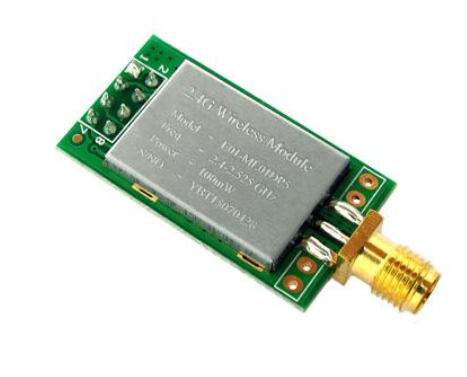
\includegraphics[width=0.4\textwidth]{Figuras/nrf24.PNG}   
	\caption{Módulo E01-ML01DP5 da EBYTE. \citep{EBYTE}}
	\label{fig:figura52}
\end{figure}


\section{Parâmetros}
\paragraph{} Para a realização da transmissão e recepção no projeto, foram usados os seguintes parâmetros do módulo E01-ML01DP5:

\begin{table}[ht]
\centering
\caption{Parâmetros do E01-ML01DP5 para o projeto.}
\vspace{0.5cm}
\begin{tabular}{r|lr}

Banda de operação & 2.400 GHz a 2.525 GHz \\
\hline
Modulação & GFSK \\
Taxa de bits & 250 \\
Potência de transmissão máxima & 20 dBm \\
Sensibilidade do receptor & -106 dBm \\
Número de canais & 126 \\
Largura de banda & 700 KHz \\
Desvio de frequência & 160 kHz \\
Alcance máximo & 2100 m
 
\end{tabular}
\label{tab:tabela2}
\end{table}

\section{\textit{MultiCeiver}}
\paragraph{} \textit{MultCeiver} é um recurso do nRF24L01+ que permite que  o receptor possa receber pacotes de até 6 endereços diferentes em paralelo, enquanto um transmissor poderá enviar apenas para 1 endereço (conforme a figura \ref{fig:figura50}). 

\begin{figure}[!ht]
	\centering
	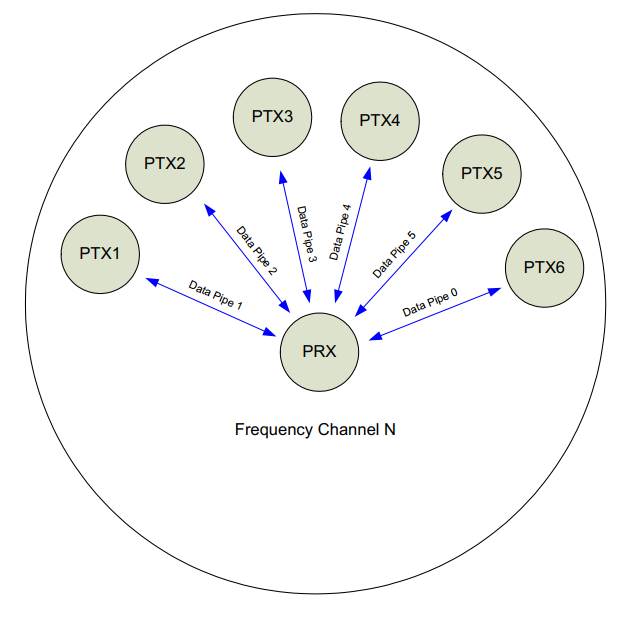
\includegraphics[width=0.4\textwidth]{Figuras/multiceiver.PNG}  
	\caption{\textit{MultiCeiver} do nRF24L01+ \citep{Nordic2008}.}
	\label{fig:figura50}
\end{figure}

\paragraph{} Como apenas um canal de dados pode receber um pacote de cada vez, a partir do momento em que um desses canais receber um pacote completo, os outros canais poderão passar a receber dados. 

\section{Estrutura dos Pacotes (Enhanced ShockBurst\textsuperscript{TM})}
\paragraph{} O pacote do nRF24L01+ segue o formato do protocolo Enhanced ShockBurst\textsuperscript{TM} que divide o pacote em preâmbulo, endereço, \textit{Packet Control}, \textit{payload} e CRC, conforme na figura \ref{fig:figura51}: 

\begin{figure}[!ht]
	\centering
	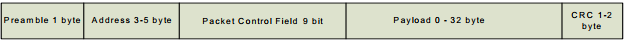
\includegraphics[width=0.7\textwidth]{Figuras/pacote_nrf24.PNG}   
	\caption{Modelo de pacote Enhanced ShockBurst\textsuperscript{TM}.\citep{Nordic2008}}
	\label{fig:figura51}
\end{figure}

\paragraph{} O preâmbulo, que serve para treinar o equalizador, apresenta um número suficiente de transições para estabilizar o receptor. Nesse formato de pacote, o preâmbulo tem apenas 1 byte contendo "10101010" se o primeiro bit do endereço for 1, ou 1 byte contendo "01010101" se o primeiro bit do endereço for 0.

\paragraph{} O segundo campo é o de endereço do receptor, ele pode ser configurado para ter de 3 a 5 bytes de tamanho. 

\paragraph{} O campo do \textit{Packet Control} apresenta 9 bits, sendo que os 6 primeiros são para definição do tamanho do payload (de "000000" a "100000"), os outros 2 bits são de \textit{Packet identification} (PID), e o último bit é para o \textit{No Acknowledgment flag} (NO\_ACK). O PID é um detector de pacote repetido, se o PID e o CRC do pacote forem iguais aos do anterior, esse pacote é considerado uma cópia e, portanto, é descartado. O nono bit do \textit{Packet Control} define se o transmissor receberá, ou não, um pacote de confirmação de recebimento.

\paragraph{} O \textit{Payload} tem tamanho dinâmico de acordo com o definido no \textit{Packet Control} e varia de 0 a 32 bytes.

\paragraph{} Por fim, o pacote disponibiliza um código CRC de 8 ou 16 bits no formato ITU-T, como citado anteriormente no capítulo 3.3.2.3 o polinômio gerador utilizado será o de 16 bits. Esse campo será preenchido com o resto da divisão da sequência de bits \textit{Packet Control} + \textit{Payload} pelo polinômio gerador.
%\chapter{STM32F411 e XBee}
\noindent

\section{Microcontrolador STM32F411}
\paragraph{} O STM32F411 é um microcontrolador baseado na arquitetura Arm Cortex-M4 e é fabricado pela STMicroelectronics. A STMicroelectronics é uma das maiores empresas de semicondutores do mundo e fica sediada na Suíça. 
a arm é a em
A arquitetura de micro controladores arm vem Se popularizando desde os anos 2000 
\pm 2018 foram produzidos mais de um bilhão de chips dessa arquitetura eph{} 



\paragraph{}
\chapter{USRP}
\section{O que é USRP?}
\paragraph{} O USRP (\textit{Universal Software Radio Peripheral}) é uma família de Rádios Definidos por \textit{Software} projetados e vendidos pela líder mundial de plataformas RDS, a Ettus Research\textsuperscript{TM} (uma empresa da National Instruments). O principal objetivo dos produtos USRP é oferecer uma alternativa de plataforma de hardware para software de rádio de valor aquisitivo mais barato. 

\paragraph{} Hoje o USRP é bastante utilizado em Laboratórios de Pesquisa e Universidades. Os produtos USRP podem ser acessados pelo PC por meio de um \textit{driver} chamado UHD, e são configurados, principalmente, por softwares como GNU Radio e \textit{LabView} da própria National Instruments, porém, também podem ser usados em outras linguagens, como a linguagem C.

\section{NI USRP-2901}
\paragraph{} Para o projeto foi utilizado o NI USRP-2901 (vide figura\ref{fig:figura90}) que é um transceptor de RF sintonizável com operação \textit{full-duplex}. Sua conexão com o PC é feita por barramento USB 2.0 ou 3.0.

\paragraph{} Esse dispositivo dispõe de 2 canais e sua faixa de operação vai de 70 MHz a 6 GHz. Sua potência máxima de saída é de 20 dBm e ele dispõe de taxa de I/Q máxima de 15 MS/s para \textit{streaming}.

\begin{figure}[!ht]
	\centering
	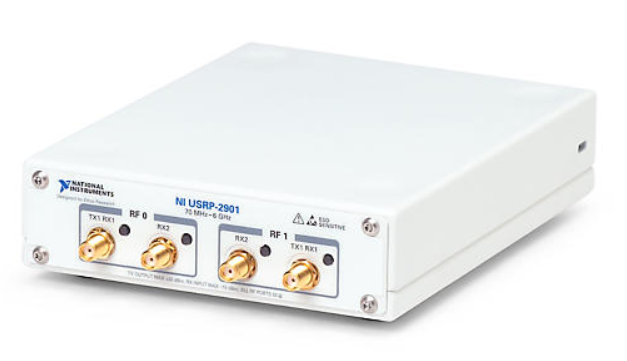
\includegraphics[width=0.4\textwidth]{Figuras/usrp.PNG}   
	\caption{NI USRP-2901 \citep{ettus}. }
	\label{fig:figura90}
\end{figure}
\chapter{Implementação}
\noindent

\paragraph{} A implementação do projeto começou com a instalação de um \textit{driver} RNDIS para microcontroladores da família STM32 ARM Cortex M4, sendo que para a implementação dessa etapa, se utilizou como base uma biblioteca criada pelo projeto Cobra 2020 da IMBEL \citep{cobra} licenciada para fins acadêmicos, que permite que o sistema do VANT possa interfacear com o modem RF, através de uma porta USB e \textit{drivers} de rede do sistema operacional, já que a referida interface é instalada pelo \textit{driver} RNDIS do SO (\textit{driver} presente nos sistemas operacionais Windows, Android e na maioria das distribuições Linux) como uma interface de rede comum. Isso foi feito para que a camada de aplicação pudesse interagir com a rede ad hoc em alto nível, de maneira genérica, da mesma forma como os celulares Android fazem ancoragem de rede USB. 

\paragraph{} A implementação ainda forneceu um servidor HTTP para configuração dos parâmetros da rede ad hoc e depuração da rede, de tal forma que essa configuração fosse feita através do navegador de um dispositivo conectado à rede.

\paragraph{} Dentro do microcontrolador foi instalada a biblioteca de código aberto da Nest \textit{Openthread} que recebe os \textit{frames} \textit{ethernet} IPv6 da camada RNDIS e faz o endereçamento dos pacotes, através do \textit{header} da subcamada MAC. Os pacotes passaram por um filtro inicial que seleciona os que são direcionados ao servidor HTTP, e não são transmitidos ao resto da rede. 

\paragraph{} Depois de passarem pela camada do \textit{OpenThread}, os pacotes foram fracionados, utilizando a biblioteca de código aberto RF24 \textit{Ethernet} que gerencia o fracionamento de até 1500 bytes em pacotes curtos de 20 bytes, que serão diretamente transmitidos pelo modem RF.

\paragraph{} Os pacotes de 20 bytes passam ainda pelo tratamento de inserção de códigos FEC, que transformam pacotes de 20 bytes em pacotes de 32 bytes, utilizando o algoritmo BCH.

\paragraph{} Para o projeto, foi elaborado um programa em linguagem C, que aplica o BCH em uma mensagem de 16 bits. Para que fosse possível enviar essa mensagem, foram introduzidos 47 bits de paridade, que gerou um código final de 63 bits. A codificação para ser do tipo \textit{“Narrow sense”} (ótima), exige uma distância de \textit{Hamming} de tamanho 23, assim podendo corrigir até 11 erros na palavra código. Para maior segurança, foi feita uma nova codificação para o projeto, a codificação de \textit{Reed-Solomon}, que também é capaz de corrigir até 11 erros em uma palavra código de 63 símbolos, porém usando apenas 22 símbolos de paridade. 

\paragraph{} Os pacotes de 32 bytes são enviados para a camada de controle do rádio nRF24L01+ que funciona em modo de transmissão \textit{broadcast} sem ACK. Em um único canal pré selecionado. Esse pacote entrega informações sobre a potência média do canal e o RSSI de cada transmissão. Para ser \textit{complience} com o protocolo IEEE 802.15.4, a estrutura de quadros utilizada pelo modem nRF24L01+ foi ajustada para se adequar a estrutura de quadro descrita no protocolo, conforme figura \ref{fig:figura80}.

\begin{figure}[!ht]
	\centering
	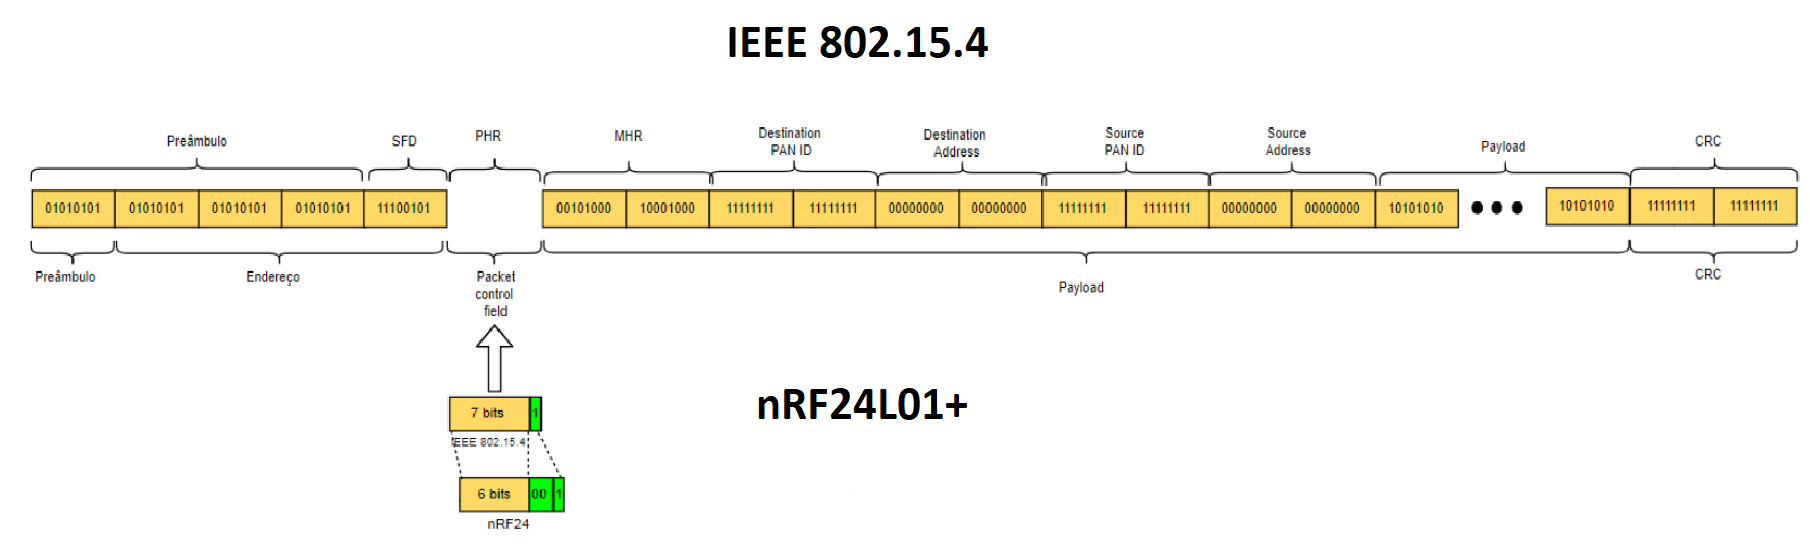
\includegraphics[width=1\textwidth]{Figuras/pacote_final.PNG}   
	\caption{Estrutura do pacote utilizado pelo projeto.}
	\label{fig:figura80}
\end{figure}

\paragraph{} Para que a adaptação representada pela figura \ref{fig:figura80} fosse possível, o nRF24L01+ precisou ser ter 4 bytes de endereço. Assim sendo, os campos PHR do IEEE 802.15.4 e o \textit{Packet Control Field} do nRF24L01+ se encontram no mesmo byte do pacote,  possibilitando que o \textit{payload} dinâmico tenha o mesmo tamanho em ambas configurações. A maior dificuldade encontrada nessa etapa foi com relação os 9 bits do \textit{Packet Control Field} que poderiam vir a dessincronizar o octeto. Para que tal não acontecesse, foi feita a expansão do campo de tamanho do nRF24L01+ para 7 bits e a compressão dos 2 bits de identificação, para que juntamente com o bit de não ACK, se tornassem apenas 1 bit. 

%\paragraph{} USRP

\paragraph{} Para gerenciar as diversas aplicações que estão sendo hospedados no microcontrolador foi utilizado um sistema operacional de tempo real, mantido pela Amazon de código aberto FreeRTOS. Cada aplicação recebe uma \textit{thread} de sistema, que gerencia o paralelismo de execução, bem como as dependências de hardware, além do uso de memória de cada aplicação. Foi utilizada também, a biblioteca de \textit{socket} do sistema operacional no interfaceamento da aplicação do servidor HTTP.  

\paragraph{} Os pacotes transmitidos foram monitorados através de uma USRP (um dispositivo RDS genérico programável) e, de um programa de linguagem gráfica G, em ambiente \textit{LabView}. Esses recursos são importantes, na medida em que monitoram o espectro RF, demodulam e decodificam os pacotes, de acordo com o protocolo IEEE 802.15.4. Vale ressaltar, que os sinais RF no canal selecionado serviram para depurar o funcionamento da rede. 

\paragraph{} Por fim, todos os códigos utilizados no desenvolvimento deste projeto foram colocados em domínio público no repositório AdHocIME git, disponível no site github.com.

%

%Foram realizados os seguintes procedimentos para se alcançar os objetivos do projeto: programação em linguagem C, para fazer a comunicação do microcontrolador com o computador via \textit{ethernet} sobre USB, recepção de pacotes enviados do nRF24L01+ por um USRP

%Dessa forma o produto final deste projeto, irá fornecer uma base para a realização da comunicação entre VANTs em uma rede Ad Hoc.

%O objetivo desse projeto é a montagem de uma rede Ad Hoc com microcontroladores que se comunicam através de um rádio RF. Para a conclusão deste objetivo, essa rede deve ser capaz de incorporar, ou excluir, dispositivos, ao se aproximarem, ou se afastarem da rede.  
\chapter{Testes e Resultados}
\noindent

\section{Materiais Utilizados}
\paragraph{} Para a realização dos testes foram usados os seguintes equipamentos:

\begin{itemize}
   \item Rádio nRF24L01+ com módulo E01-ML01DP5.
   \item Rádio NI USRP-2901 da Ettus Research.
   \item Microcontrolador STM32F411 da STM.
   \item Antenas.
   \item Software \textit{LabView}.
   \item Software \textit{MatLab}.
   \item N9938A Analisador de Espectros de Micro-ondas de Mão FieldFox da Keysight Technologies.
\end{itemize}

\section{Definição de Parâmetros}
\paragraph{} De acordo com o estudo dos padrões IEEE 802.15.4 e nRF24L01+ definimos diversos parâmetros que foram utilizados no projeto. 

\paragraph{} Primeiramente,  a frequência central de 2,515 GHz foi estabelecida para evitar a interferência de outros dispositivos que utilizam a faixa ISM de 2,4 Ghz. Também foi escolhida a taxa de bits da transmissão, e essa é de 250 kbps.

\paragraph{} Em relação às configurações do pacote, foram definidos, como citado anteriormente no capítulo 9, o número de bytes do endereço do rádio e que o pacote terá \textit{payload} dinâmico. No \textit{Packet Control Field} também será definido como 1 o bit de \textit{NO\_ACK}, significando que a transmissão não terá pacote de confirmação de entrega.

\paragraph{} Também foram definidos os campos de configuração do \textit{Frame Control} conforme mostra a figura \ref{fig:figura99}. O primeiro campo de configuração é o \textit{Security Enabled}, e seu bit receberá o valor 0, a fim de desabilitar a segurança da subcamada MAC, pois toda parte de segurança da informação estará a cargo da codificação e do \textit{OpenThread}. Igualmente ao campo de \textit{NO\_ACK}, o AR não será habilitado, então será preenchido com o bit 0. 

\paragraph{} Como o \textit{OpenThread} trabalha com pacotes IEEE 802.15.4 de 2006, sua versão será designada com os bits "01", e seus campos de \textit{Sequence Number Suppression} e \textit{IE present} serão 1 e 0 respectivamente. Além desses campos, a versão de 2006 também especifica que o \textit{PAN ID Compression} será 0, devido ao fato de \textit{OpenThread} exigir o PAN ID do destino e da fonte. Por fim, os endereços do receptor e do transmissor serão de apenas de 2 bytes, então os campos de \textit{Addressing Mode} vão ser iguais a "10".

\begin{figure}[!ht]
	\centering
	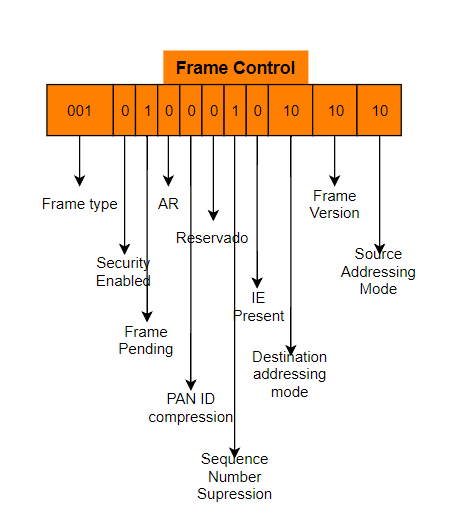
\includegraphics[width=0.4\textwidth]{Figuras/MHR.PNG}   
	\caption{Configuração do \textit{Frame Control}}
	\label{fig:figura99}
\end{figure}


\section{Testes com Ping}
\paragraph{} Para testar a classe RNDIS de \textit{driver} USB embarcado no microcontrolador foi utilizado a pilha TCP/IP do SO de tempo real FreeRTOS. Esse sistema operacional vem com uma aplicação pronta de servidor ping, o qual pode ser visto na figura \ref{fig:figura100} respondendo um teste com a placa conectada a um PC de sistema operacional Windows. 

\paragraph{} Na imagem \ref{fig:figura101} podemos ver a interface de rede virtual criada em um sistema operacional Windows pelo \textit{driver} da classe USB do RNDIS. O endereço IP, endereço de \textit{gateway} e endereço de DNS foram configurados através de interface do SO Windows. Sendo que o endereço MAC detectado é idêntico ao endereço configurado no microcontrolador.  

\begin{figure}[!ht]
	\centering
	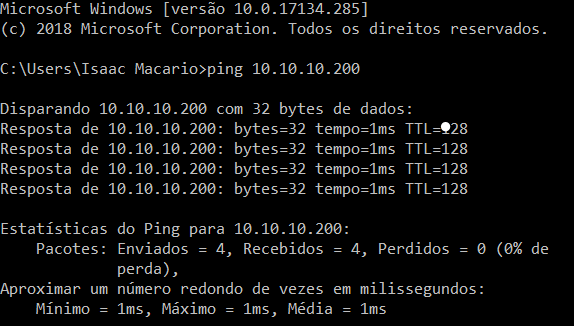
\includegraphics[width=0.4\textwidth]{Figuras/ping.PNG}   
	\caption{Ping na rede}
	\label{fig:figura100}
\end{figure}

\begin{figure}[!ht]
	\centering
	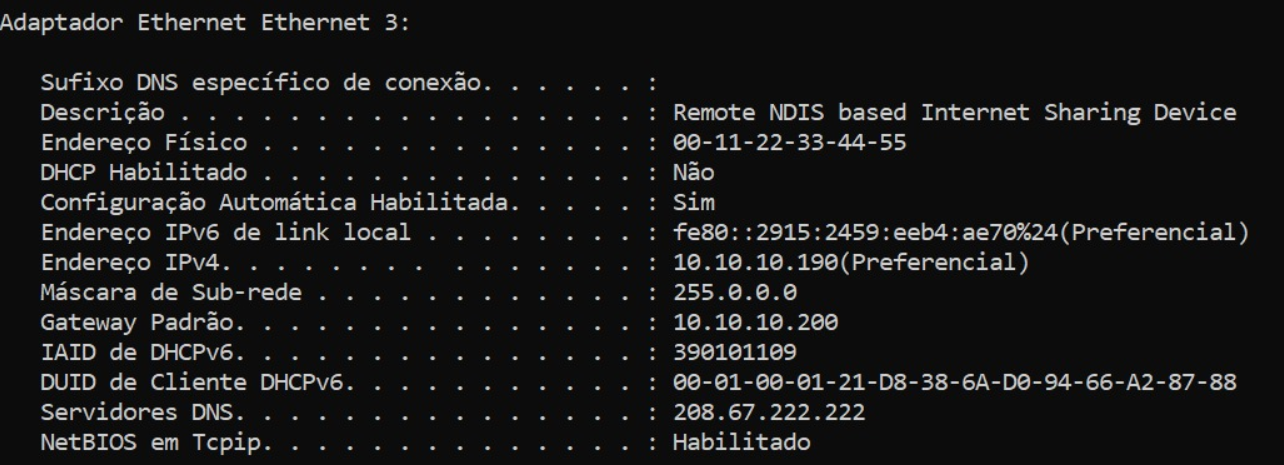
\includegraphics[width=0.5\textwidth]{Figuras/ipconfig.PNG}   
	\caption{Ipconfig}
	\label{fig:figura101}
\end{figure}

\section{Testes com o Servidor HTTP}

\paragraph{} O servidor HTTP foi desenvolvido a partir da biblioteca de \textit{socket} do sistema operacional \textit{FreeRTOS}. Como teste, foi escrita uma página HTML, na qual é possível através de \textit{inputs} de texto definir o estado dos LEDs na placa. De forma a acender e apagar os LEDs da placa de desenvolvimento foi utilizada através de uma página no \textit{browser} do computador, no qual a placa está ligada.
Foi desenvolvida uma aplicação de teste para validar o funcionamento do servidor HTTP (vide figura \ref{fig:figura150}).  

\FloatBarrier
\begin{figure}[!htp]
\centering
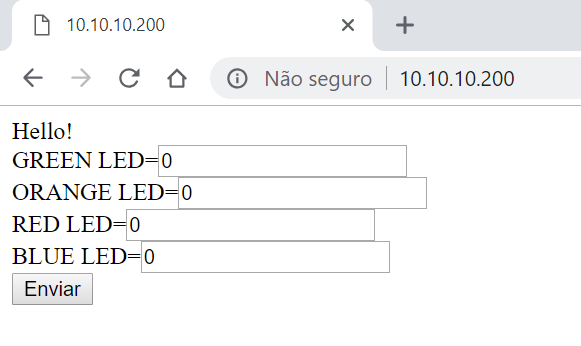
\includegraphics[scale = 0.8]{Figuras/httpServer.PNG}
\caption{Servidor HTTP}
\label{fig:figura150}
\end{figure}
\FloatBarrier

\section{Testes de Transmissão e Recepção de Pacotes}

\paragraph{} Utilizamos uma biblioteca de código aberto disponível na comunidade em repositório git do site GitHub \citep{gitnrf}  para uso com o modem NRF24L01+, para teste do porte da biblioteca para o microcontrolador utilizado no projeto, foi desenvolvida uma aplicação de exemplo em que o transmissor a cada um segundo transmitia um pacote de dados e piscava um LED da placa. Enquanto o receptor a cada pacote recebido piscava outro LED da placa.

\paragraph{} Quando transmissor e receptor foram ligados ao mesmo tempo os LEDs das duas placas piscaram em sincronia completando o teste dos modens. 


\section{Recepção de Pacotes nRF24L01+ com o USRP}
\paragraph{} Para testar a capacidade de transmissão do rádio nRF24L01+ foram feitos os seguintes procedimentos: 

\begin{itemize}
    \item Carregou-se o STM32F411 com o programa feito em linguagem C \citep{gitnrf} que configura o nRF24L01+ de acordo com as especificações requeridas no projeto, de forma que a cada 1 segundo seja transmitido um sinal RF. A figura \ref{fig:figura103} representa a conexão entre o microcontrolador e o rádio para poder realizar a transmissão.
    
    \begin{figure}[!ht]
	\centering
	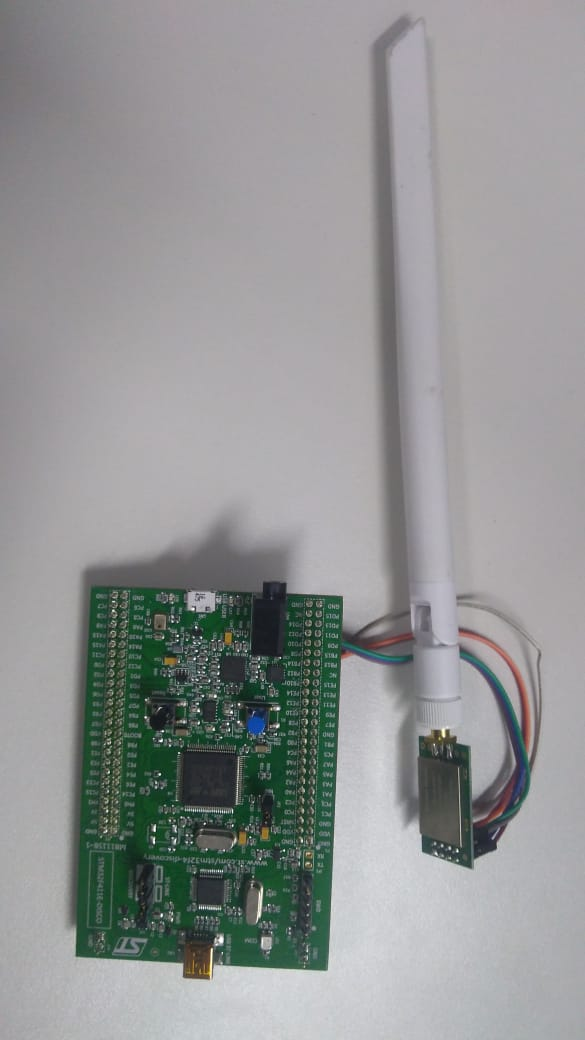
\includegraphics[width=0.4\textwidth, angle=90]{Figuras/stm_radio.jpeg}   
	\caption{STM32F411 conectado ao nRF24L01+.}
	\label{fig:figura103}
    \end{figure}
    
    \item Para a validação da transmissão de um sinal, foi usado o espectrômetro citado da seção 10.1 e o resultado pode ser visto pela figura \ref{fig:figura104}, que apresenta uma transmissão com frequência central em 2,515 GHz.
    
    \begin{figure}[!ht]
	\centering
	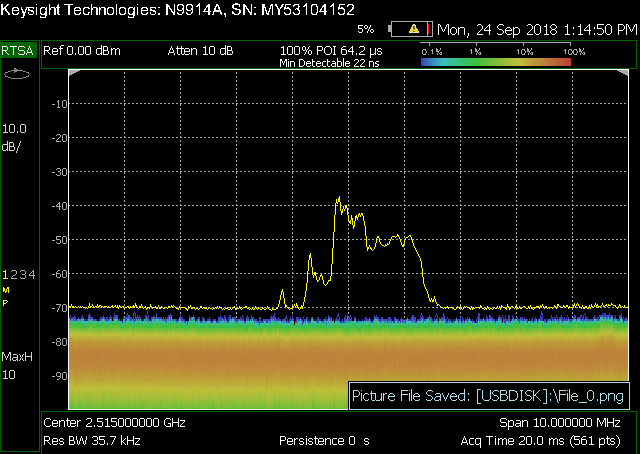
\includegraphics[width=0.5\textwidth]{Figuras/File_01.png}  
	\caption{Resultado no analisador de espectros.}
	\label{fig:figura104}
    \end{figure}

\begin{comment}    
    \item Por fim, foi utilizado o rádio USRP como um receptor do sinal RF enviado pelo nRF24L01+. O USRP foi configurado com o \textit{software} LabView de forma que sua taxa de IQ chegasse a 5000000 amostras por segundo quando a relação amostras por símbolo for igual a 2, além disso o projeto do LabView também faz a demodulação FSK-2 do sinal, de forma a reconstruir os bits transmitidos. As representações dessa demodulação são representadas pelas figuras \ref{fig:figura105} e \ref{fig:figura106}. 

\begin{figure}    
    \centering
    
        \begin{subfigure}[b]{0.4\textwidth}
        	\includegraphics[width=\textwidth]{Figuras/.PNG}   
        	\caption{}
        	\label{fig:figura105}
        \end{subfigure}
    
        \begin{subfigure}[b]{0.4\textwidth}
        	\includegraphics[width=\textwidth]{Figuras/.PNG}   
        	\caption{}
        	\label{fig:figura106}
        \end{subfigure}
    
    \caption{Projeto em LabView}\label{fig:animals}
\end{figure}
    
\end{comment} 

\end{itemize}


\section{Simulações para Dimensionamento do Enlace}
\paragraph{}As simulações para o dimensionamento do enlace foram realizadas utilizando o software MatLab, sendo aplicado o modelo de 2 raios. Os principais parâmetros utilizados foram: altura da antena transmissora $h_t = 40m$, altura da antena receptora $h_r = 40m$, distância entre as antenas $d = 2000m$, frequência de operação $\textit{f} = 2.4GHz$, ganho máximo das antenas $G_{max} = 2.15dB$, condutividade do solo $\sigma = 0.005 S/m$, potência transmitida $P_t = 20 dBm$, permissividade relativa do solo típico $\epsilon_r = 15$, desvio padrão das irregularidades de altura $\Delta h = 0.3m$ e sensibilidade da antena receptora de -86 dBm. As ondas que estão se propagando com polarização perpendicular.

\paragraph{}Para esse esses parâmetros, a fronteira para a região de campo distante está localizada a $R = 0,0625m$ da antena transmissora, podendo considerar as frentes de onda planas a partir dessa distância. A distância de horizonte calculada foi $d_h = 26.030,751m$
e a fronteira entre a zona de interferência e difração foi $d_0 = 153.600m$. Portanto, como o enlace analisado se encontra na zona de interferência do sistema, e o modelo de terra plana para 2 raios pode ser utilizado.

\FloatBarrier
\begin{figure}[!htp]
\centering
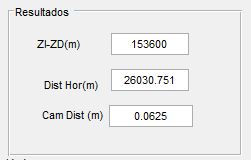
\includegraphics[scale = 0.8]{Figuras/Parametros.JPG}
\caption{}
\end{figure}
\FloatBarrier

\paragraph{}O dimensionamento do enlace realizado foi feito para analisar as influências da atenuação do espaço livre, do coeficiente de reflexão, da rugosidade do solo e, da diretividade das antenas.

\paragraph{}A primeira análise que foi feita, levou em consideração somente o efeito do modelo de 2 raios. A atenuação no espaço livre, a rugosidade do solo, o coeficiente de reflexão e a diretividade das antenas foram descartadas. Assim, foi obtido:

\FloatBarrier
\begin{figure}[!htp]
\centering
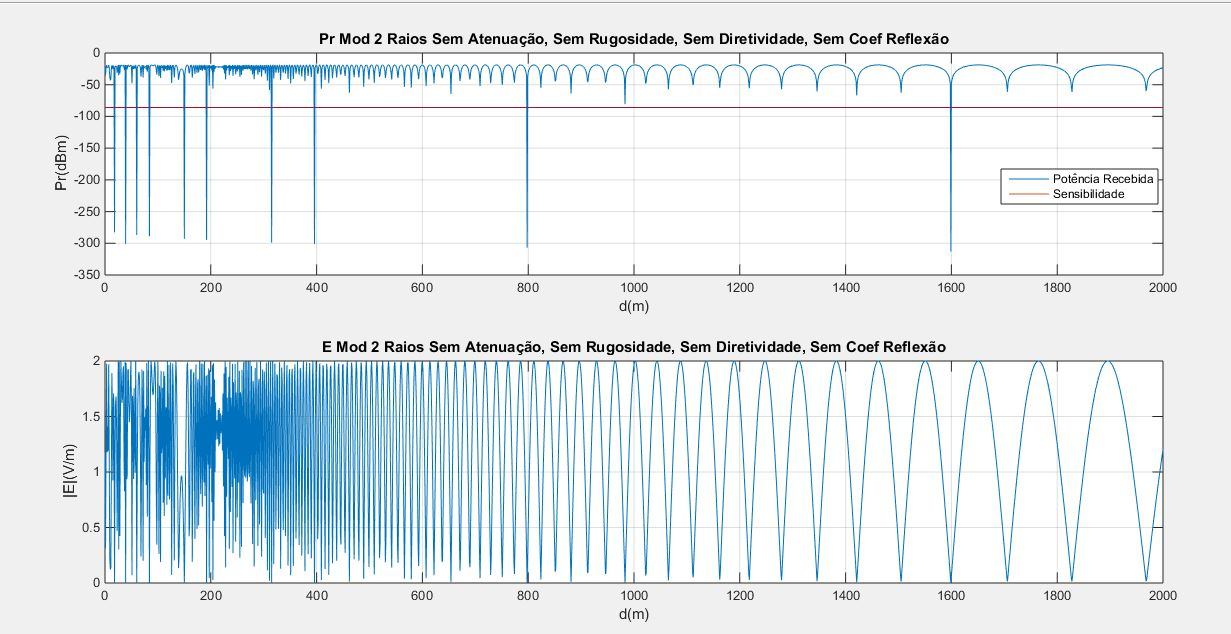
\includegraphics[scale = 0.3]{Figuras/SA_SR_SD_SCR.JPG}
\caption{Potência Recebida e Campo Elétrico na antena receptora, respectivamente, sem atenuação, sem rugosidade, sem diretividade e sem coeficiente de reflexão.}
\end{figure}
\FloatBarrier

\paragraph{}Nesse primeiro gráfico é possível constatar a grande oscilação existente, tanto no campo elétrico, quanto na potência recebida. Tal oscilação se justifica pelo fato das antenas se encontrarem na região de interferência do enlace. Os valores de menor potência, são alternados, devido as interferências destrutivas e construtivas, entre o campo elétrico direto e o refletido. Os picos negativos que ultrapassam a sensibilidade da antena receptora, são pontos em que o campo elétrico resultante é nulo, enquanto que, os outros valores mínimos da potência que se repetem, são  valores em que, o módulo do campo elétrico é baixo, mas diferente de zero.

\paragraph{}Agora será analisado somente o efeito da atenuação no enlace. Nessa situação, temos que:



\FloatBarrier
\begin{figure}[!htp]
\centering
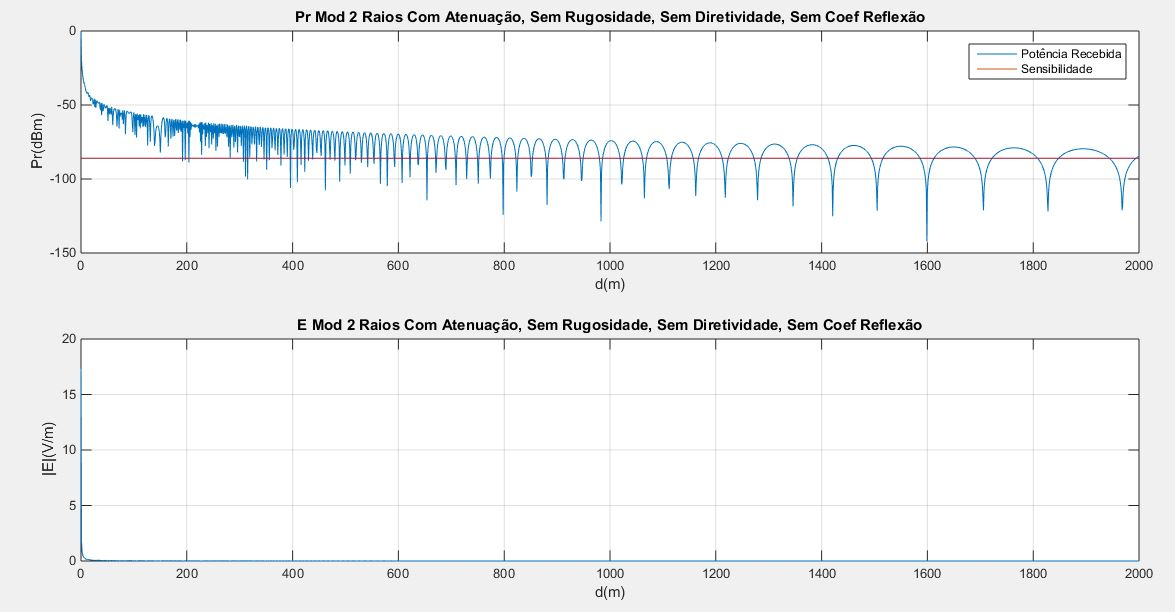
\includegraphics[scale = 0.3]{Figuras/CA_SR_SD_SCR.JPG}
\caption{Potência Recebida e Campo Elétrico na antena receptora, respectivamente, com atenuação, sem rugosidade, sem diretividade e sem coeficiente de reflexão.}
\end{figure}
\FloatBarrier

\paragraph{}Podemos observar, que a atenuação no espaço livre apresenta uma grande influência na potência recebida pela antena. Ao se analisar o campo elétrico mais detalhadamente, temos que:

\FloatBarrier
\begin{figure}[!htp]
\centering
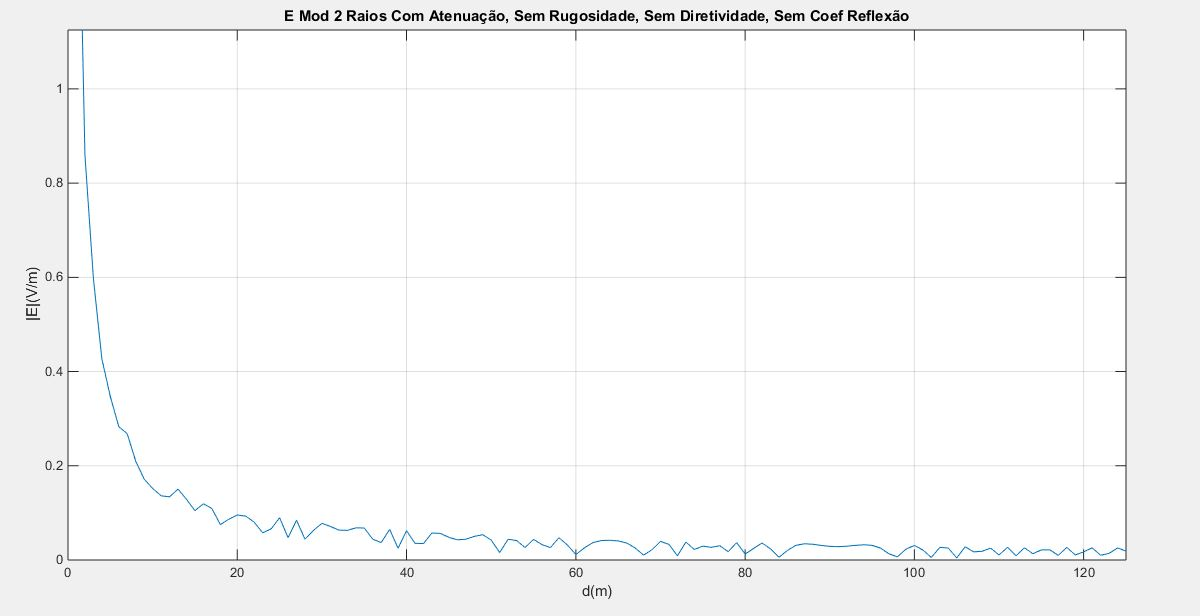
\includegraphics[scale = 0.3]{Figuras/CA_SR_SD_SCR_E.JPG}
\caption{Campo Elétrico na antena receptora, com atenuação, sem rugosidade, sem diretividade e sem coeficiente de reflexão.}
\end{figure}
\FloatBarrier

\paragraph{}Assim sendo, observamos que para pequenas distâncias, o valor do campo elétrico resultante já é bastante atenuado, o que faz com que para uma distância de aproximadamente $d = 200m$, existam pontos em que a potência se torna menor do que a sensibilidade. E, à medida em que a distância aumenta, a potência diminui cada vez mais.

\paragraph{}O próximo fator a ser analisado será o da rugosidade. Levando em consideração somente esse fator, obtivemos o seguinte gráfico:

\FloatBarrier
\begin{figure}[!htp]
\centering
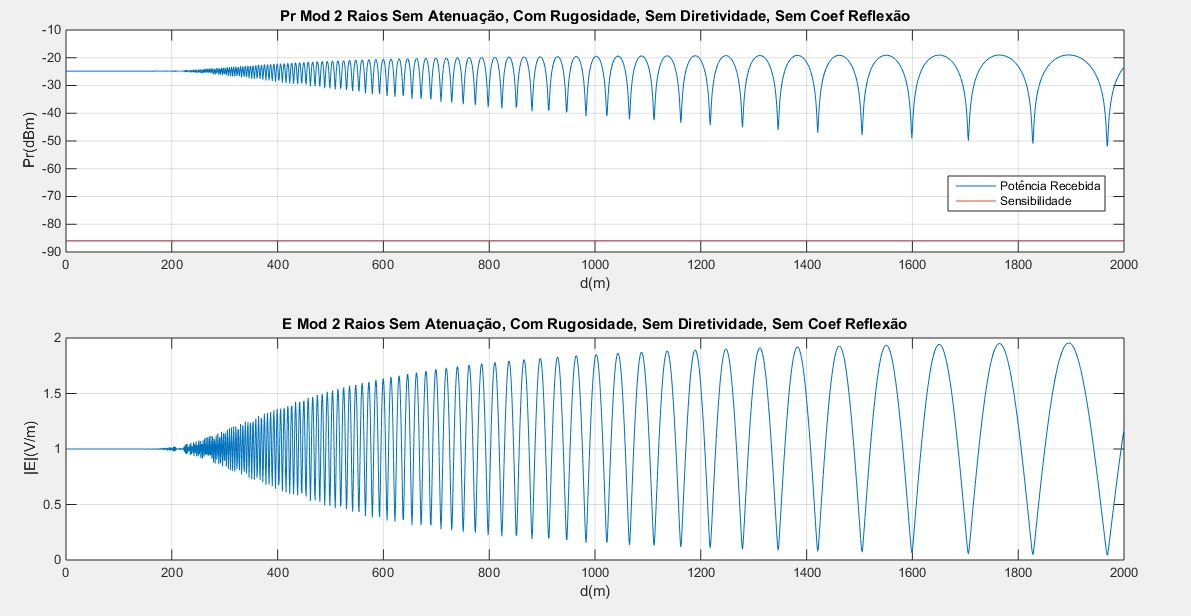
\includegraphics[scale = 0.3]{Figuras/SA_CR_SD_SCR.JPG}
\caption{Potência Recebida e Campo Elétrico na antena receptora, respectivamente, sem atenuação, com rugosidade, sem diretividade e sem coeficiente de reflexão.}
\end{figure}
\FloatBarrier

\paragraph{}Nesse gráfico percebemos que para uma distância entre as antenas de aproximadamente até $d = 200m$ aproximadamente, toda a oscilação existente, devido a zona de interferência, foi eliminada. A expressão \ref{Mod2Raios}, mostra a dependência do campo elétrico do fator de espalhamento $\rho_s$. Para se entender melhor como foi o comportamento desse fator, ao longo do enlace analisado, construímos o seguinte gráfico:

\FloatBarrier
\begin{figure}[!htp]
\centering
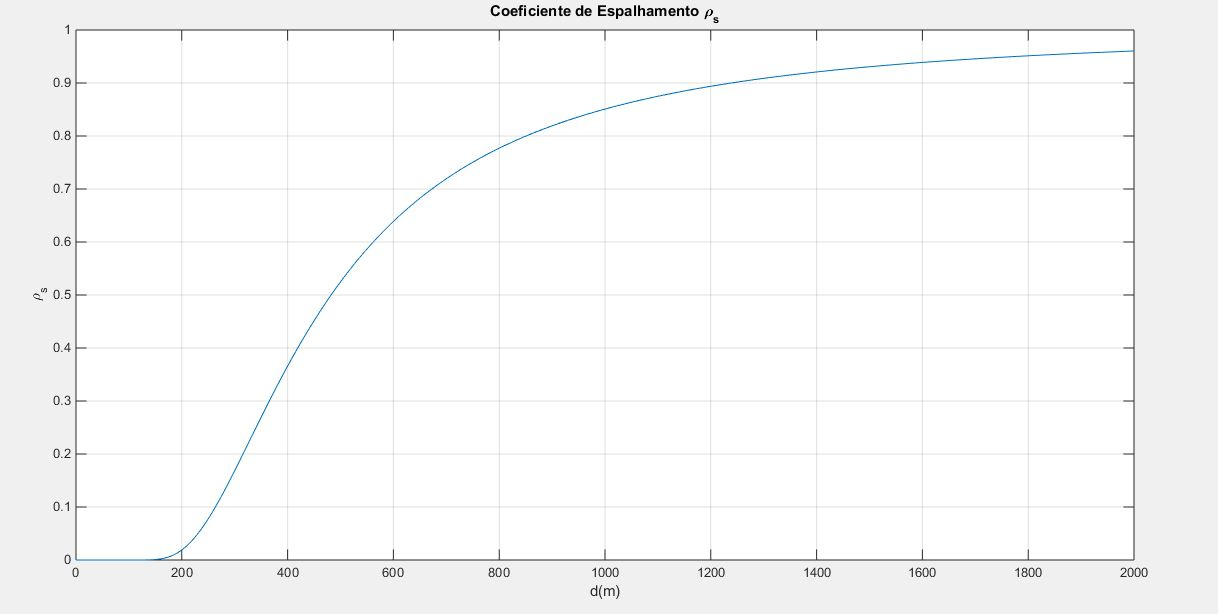
\includegraphics[scale = 0.3]{Figuras/Coef_Espalha_2.JPG}
\caption{Coeficiente de Espalhamento $\rho_s$.}
\end{figure}
\FloatBarrier

\paragraph{}Assim, o coeficiente de espalhamento atenua bastante a componente do campo elétrico refletido no solo, porque ele é nulo nessa região, que vai até $d = 200m$ aproximadamente. A partir dessa distância, $\rho_s$ começa a ser diferente de zero, permitindo que a componente do campo elétrico que é refletido no solo comece a ter uma influência mensurável na medida da potência recebida pela antena receptora, fazendo com que ocorram as interferências tanto construtivas, como destrutivas, que são características desse modelo.

\paragraph{}O próximo gráfico mostra a influência somente das funções direcionais das antenas $F(\theta)$. São influências no campo elétrico, por conseguinte, na potência recebida, também podem ser vistas na expressão \ref{Mod2Raios}. Na simulação, as funções direcionais das antenas obedecem a seguinte expressão:

\begin{equation}
\label{F}
    F(\theta) = \sqrt{G(\theta)}
\end{equation}

\paragraph{}Onde $G(\theta)$ é o ganho da antena.

\paragraph{}Sendo assim, o gráfico obtido foi:



\FloatBarrier
\begin{figure}[!htp]
\centering
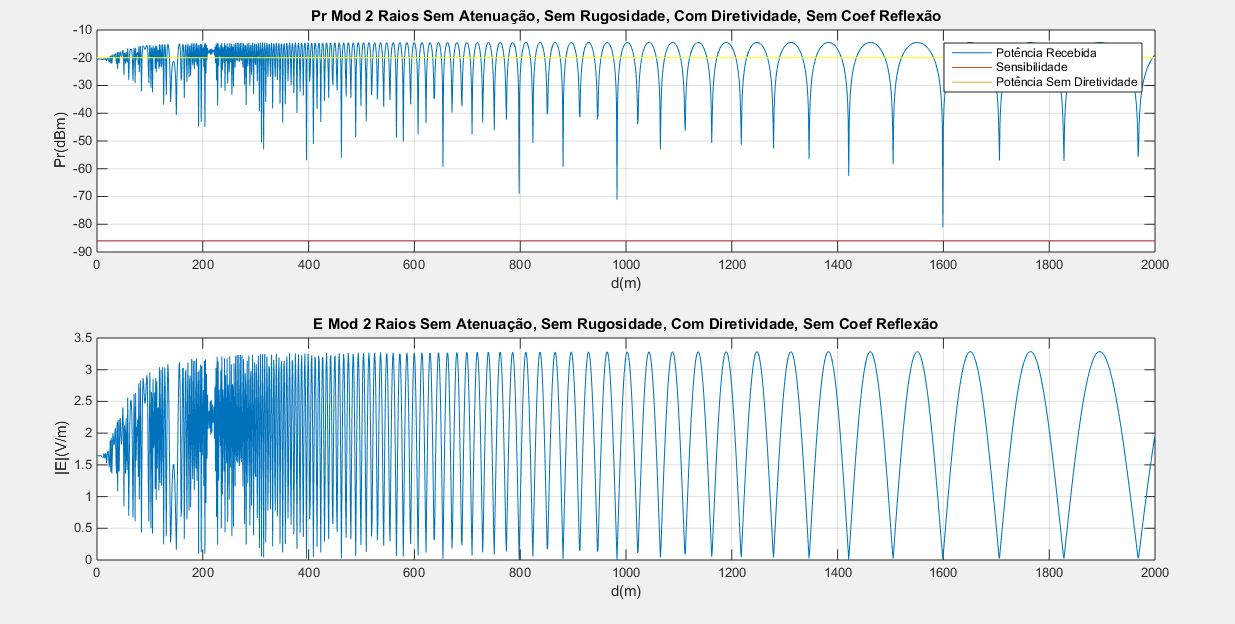
\includegraphics[scale = 0.3]{Figuras/SA_SR_CD_SCR_2.JPG}
\caption{Potência Recebida e Campo Elétrico na antena receptora, respectivamente, sem atenuação, sem rugosidade, com diretividade e sem coeficiente de reflexão.}
\label{Diretividade}
\end{figure}
\FloatBarrier

\paragraph{}Nesse gráfico vemos que houve um ganho em relação ao cenário inicial, oque pode ser visto na figura \ref{Diretividade}. A linha amarela superior indica o limiar superior da potência numa situação onde a diretividade não é levada em consideração. Outra conclusão a que se pode chegar é que, para distâncias bem pequenas entre as antenas, há uma atenuação do campo elétrico, enquanto que à medida que elas se afastam, o campo elétrico, e, consequentemente, a potência no receptor passam a sofrer ganhos. Isso ocorre devido as funções direcionais das antenas, que se comportam de acordo com o seguinte gráfico:


\FloatBarrier
\begin{figure}[!htp]
\centering
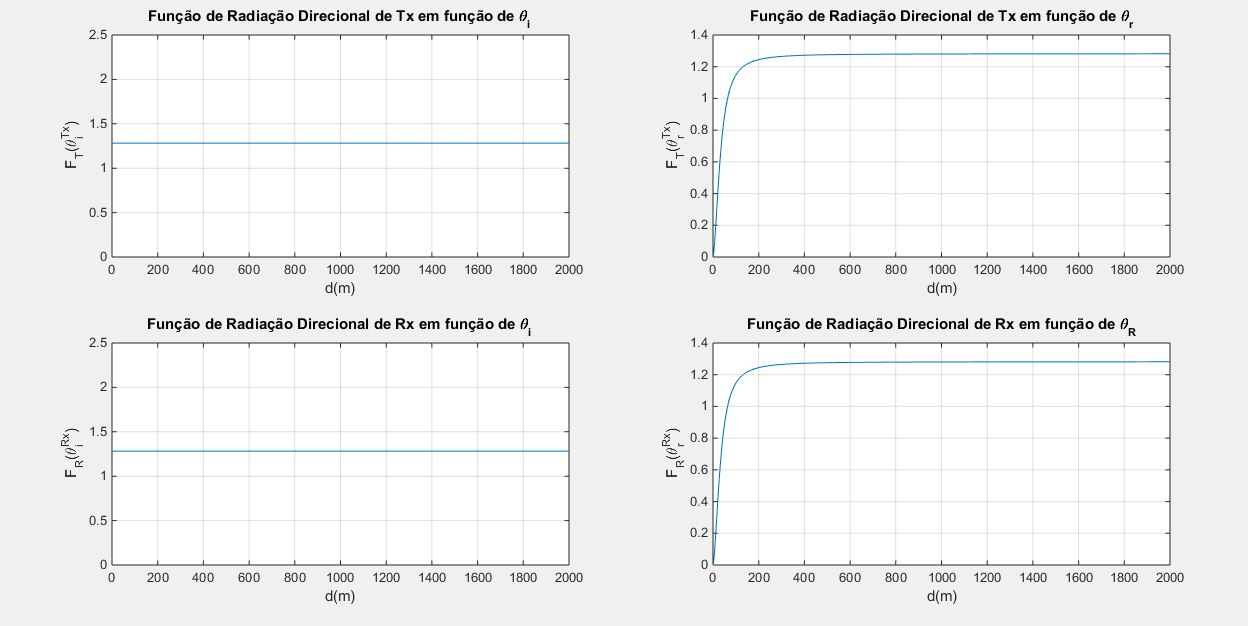
\includegraphics[scale = 0.3]{Figuras/Funcao_Radiacao_Direcional.JPG}
\caption{Funções de Radiação Direcional das antenas.}
\end{figure}
\FloatBarrier

\paragraph{}Pelas expressões \ref{Ganho} e \ref{F}, temos que as equações de radiação direcional das antenas estão em função da raiz quadrada de $\sin^3 \theta$. As $F_T(\theta_i^{Tx})$ e $F_R(\theta_i^{Rx})$ são funções direcionais referentes ao ângulo de radiação do campo direto, que não sofrem reflexão. Como as antenas estão na mesma altura, elas são constantes para todas as distâncias, e iguais ao seu valor máximo, pois $\theta = 90\degree$ com a vertical. Já as funções direcionais de radiação referentes ao campo elétrico refletido, $F_T(\theta_r^{Tx})$ e $F_R(\theta_r^{Rx})$, apresentam valores baixos para distâncias pequenas, onde $\theta_r^{Tx} \approx 180\degree$, para a antena transmissora, e $\theta_r^{Rx} \approx 0\degree$ para a antena receptora, onde $\theta_r^{Tx}$ e $\theta_r^{Rx}$, são os ângulos referentes ao campo refletido radiados pela antena transmissora e receptora respectivamente, onde os ângulos são medidos em relação a vertical. A medida em que as antenas se afastam, os ângulos  $\theta_r^{Tx}$ e $\theta_r^{Rx}$ se aproximam de $90\degree$ e por isso, os valores das funções vão aumentando com a distância, proporcionando o ganho de potência visto na figura \ref{Diretividade}.

\paragraph{}Agora vejamos como o coeficiente de reflexão influencia no valor da potência recebida pela antena receptora. Os gráficos obtidos foram:


\FloatBarrier
\begin{figure}[!htp]
\centering
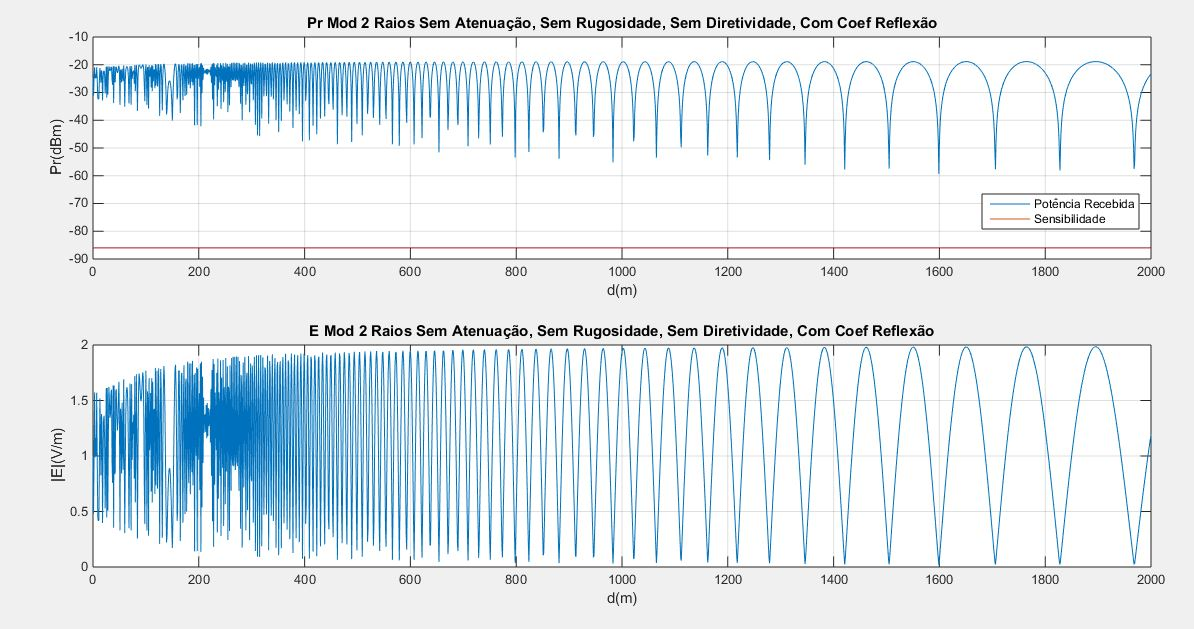
\includegraphics[scale = 0.3]{Figuras/SA_SR_SD_CCR.JPG}
\caption{Potência Recebida e Campo Elétrico na antena receptora, respectivamente, sem atenuação, sem rugosidade, sem diretividade e com coeficiente de reflexão.}
\end{figure}
\FloatBarrier

\paragraph{}Tendo como referência a expressão \ref{Mod2Raios}, o coeficiente de reflexão tem uma influência semelhante ao do coeficiente de espalhamento $\rho_s$. Vejamos como $\Gamma(\theta_i)$, varia de acordo com o ângulo de incidência $\theta_i$:

\FloatBarrier
\begin{figure}[!htp]
\centering
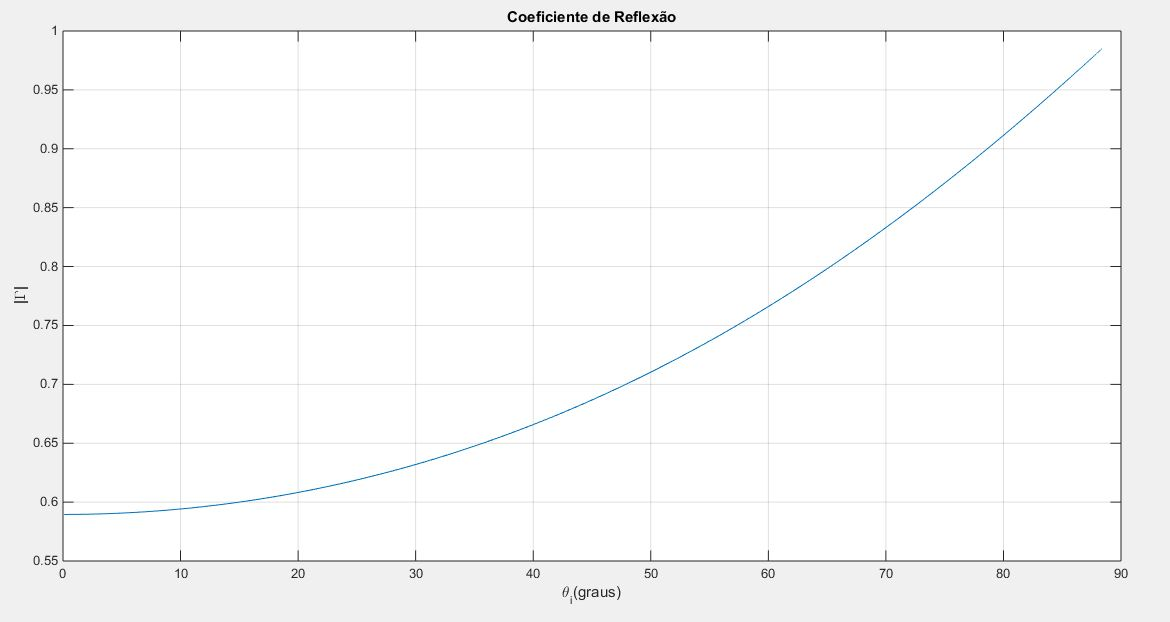
\includegraphics[scale = 0.3]{Figuras/Coef_Ref.JPG}
\caption{Coeficiente de Reflexão $\Gamma$}
\end{figure}
\FloatBarrier

\paragraph{}Logo, vemos que o coeficiente de reflexão atenua um pouco o campo elétrico refletido, para ângulos de incidência menores, o que ocorre quando as antenas estão muito próximas. À medida em que as antenas se afastam, o ângulo de incidência se aproxima de $90\degree$, e essa atenuação diminui. Em relação a potência, ela está sempre acima da sensibilidade.

\paragraph{}Por fim, analisaremos o gráfico que apresenta a potência recebida na antena receptora, e o módulo do campo elétrico da mesma com todos os fatores, atenuação, rugosidade, diretividade e coeficiente de reflexão - levados simultaneamente em consideração. Assim:

\FloatBarrier
\begin{figure}[!htp]
\centering
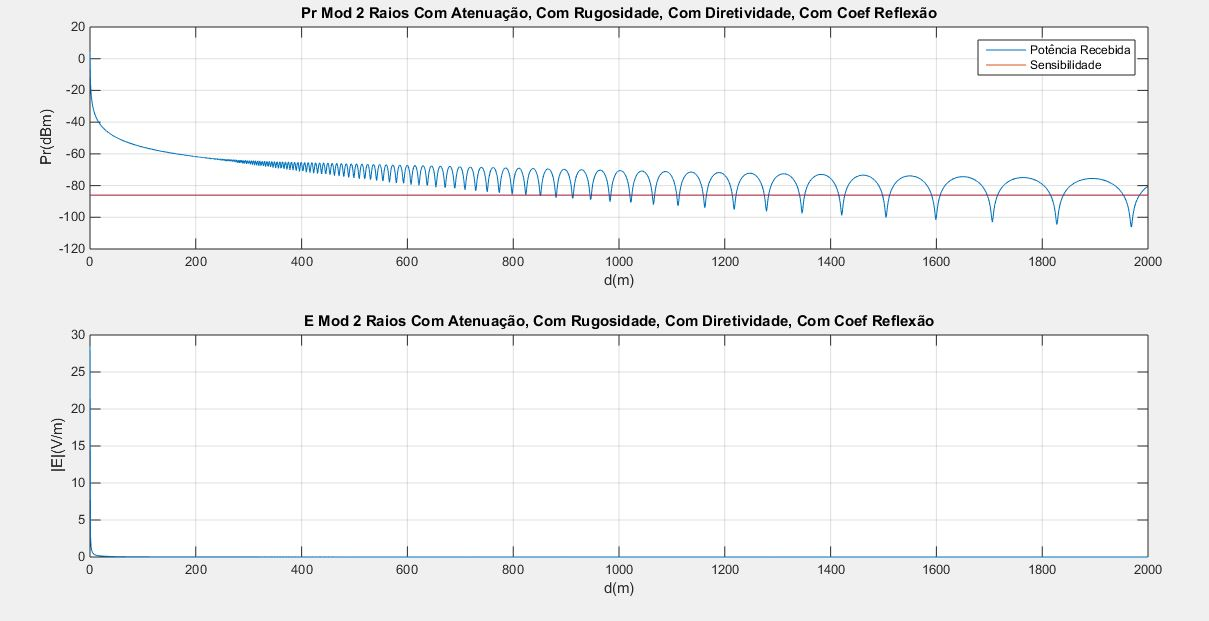
\includegraphics[scale = 0.3]{Figuras/CA_CR_CD_CCR.JPG}
\caption{Potência Recebida e Campo Elétrico na antena receptora, respectivamente, com atenuação, com rugosidade, com diretividade e com coeficiente de reflexão.}
\label{completo_1}
\end{figure}
\FloatBarrier

\FloatBarrier
\begin{figure}[!htp]
\centering
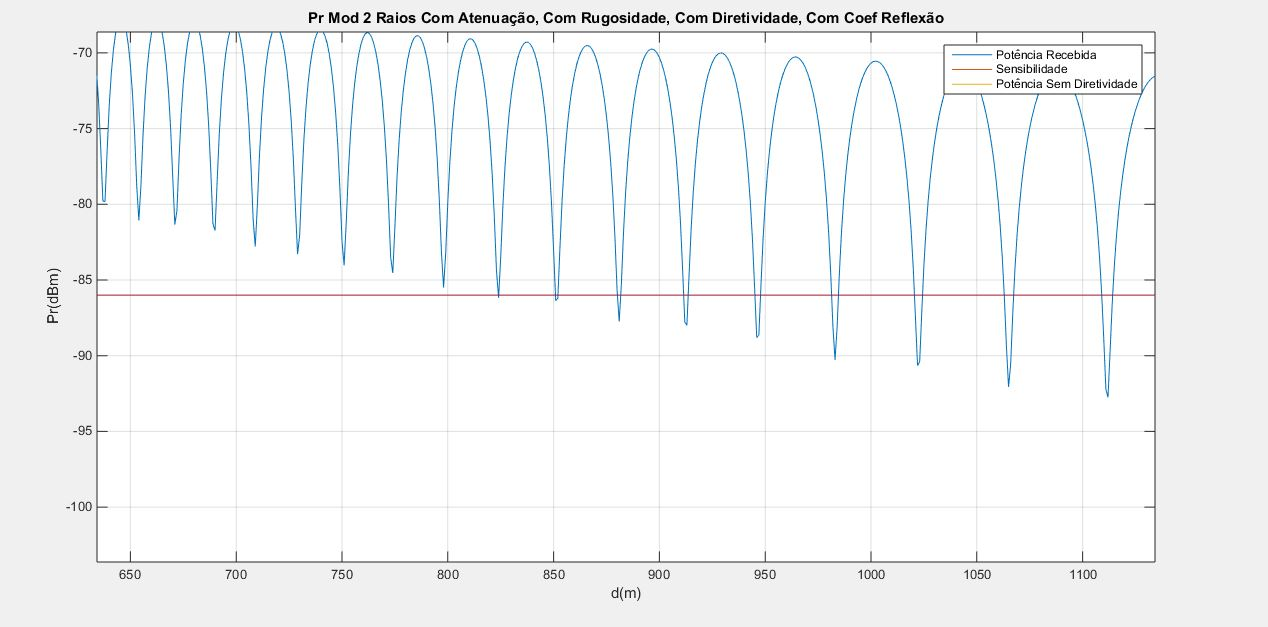
\includegraphics[scale = 0.3]{Figuras/CA_CR_CD_CCR_2.JPG}
\caption{Potência Recebida na antena receptora, respectivamente, com atenuação, com rugosidade, com diretividade e com coeficiente de reflexão.}
\label{completo_2}
\end{figure}
\FloatBarrier

\FloatBarrier
\begin{figure}[!htp]
\centering
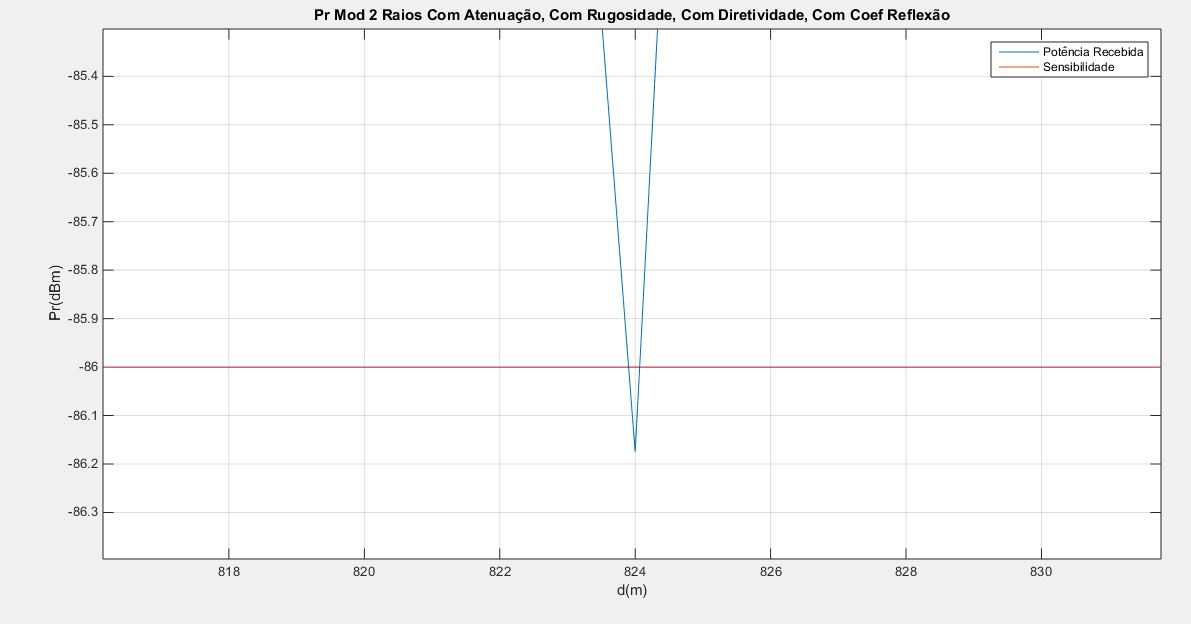
\includegraphics[scale = 0.3]{Figuras/CA_CR_CD_CCR_4.JPG}
\caption{Região onde a potência recebida está abaixo da sensibilidade pela primeira vez.}
\label{completo_2}
\end{figure}
\FloatBarrier

\paragraph{}Assim sendo, vemos que nessa situação, a potência é bastante reduzida, principalmente pela atenuação do espaço livre, permitindo que haja uma garantia de comunicação entre os VANTs numa distância que pode ser de até $d \approx 824m$ conforme mostra a figura \ref{completo_2}. A partir daí, o número de pontos onde a potência recebida é menor do que a sensibilidade se torna maior a medida que as antenas se afastam.

\paragraph{}É importante ressaltar o fato das antenas estarem a mesma altura, pois essa é melhor condição possível para o nosso enlace. Isso pode ser percebido pelo próximo gráfico, que mostra como a potência varia de acordo com a variação da altura da antena receptora $20m \leq h_r \leq 60m$ e $h_t = 40m$ separadas de uma distância de 100m.

\FloatBarrier
\begin{figure}[!htp]
\centering
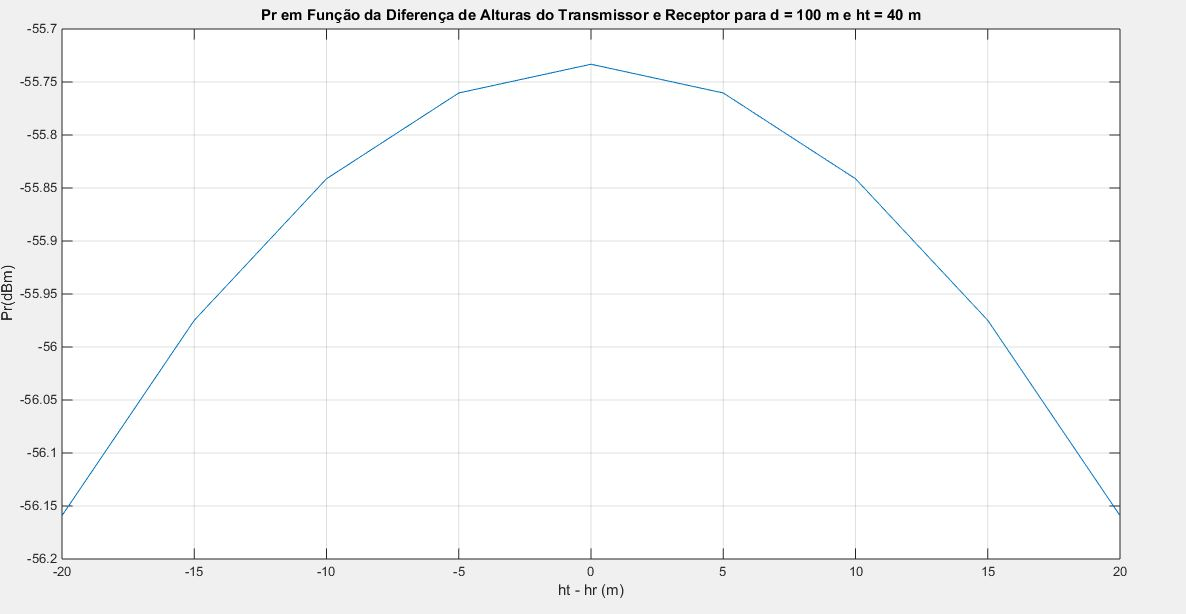
\includegraphics[scale = 0.3]{Figuras/Diferenca_Altura.JPG}
\caption{Potência Recebida na antena receptora, respectivamente, com atenuação, com rugosidade, com diretividade e com coeficiente de reflexão, em função da diferença de alturas entre antena transmissora e receptora.}
\end{figure}
\FloatBarrier

\paragraph{}E nesse contexto no qual as antenas apresentam a mesma altura, foi construído o seguinte gráfico:

\FloatBarrier
\begin{figure}[!htp]
\centering
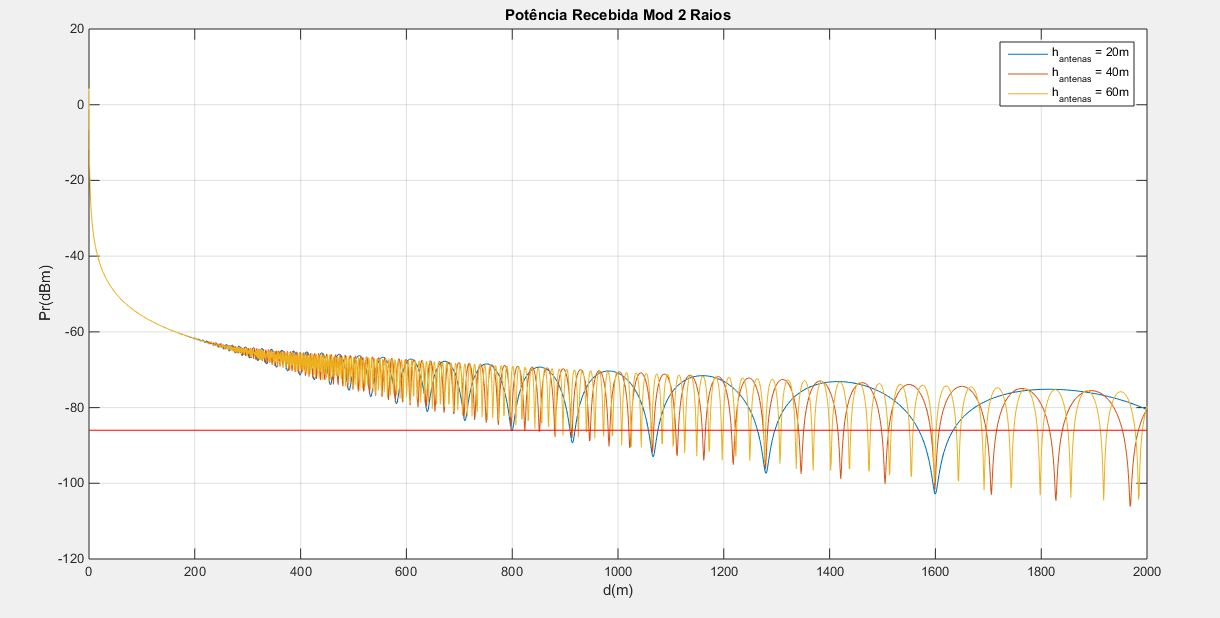
\includegraphics[scale = 0.3]{Figuras/Mesma_Altura.JPG}
\caption{Potência Recebida na antena receptora, estando as antenas a mesma altura, com atenuação, com rugosidade, com diretividade e com coeficiente de reflexão.}
\end{figure}
\FloatBarrier

\paragraph{}Dessa forma, vê-se que o melhor cenário para o enlace é aquele no qual a altura é a menor possível, pois a oscilação é menor num mesmo intervalo de distância, quando comparado a potência onde as alturas das antenas são maiores, resultando, assim, num menor número de vezes que a potência na antena receptora fica abaixo da sensibilidade.


\paragraph{}A potência recebida na antena receptora para duas antenas que estão a 20m do solo se comporta da seguinte maneira:

\FloatBarrier
\begin{figure}[!htp]
\centering
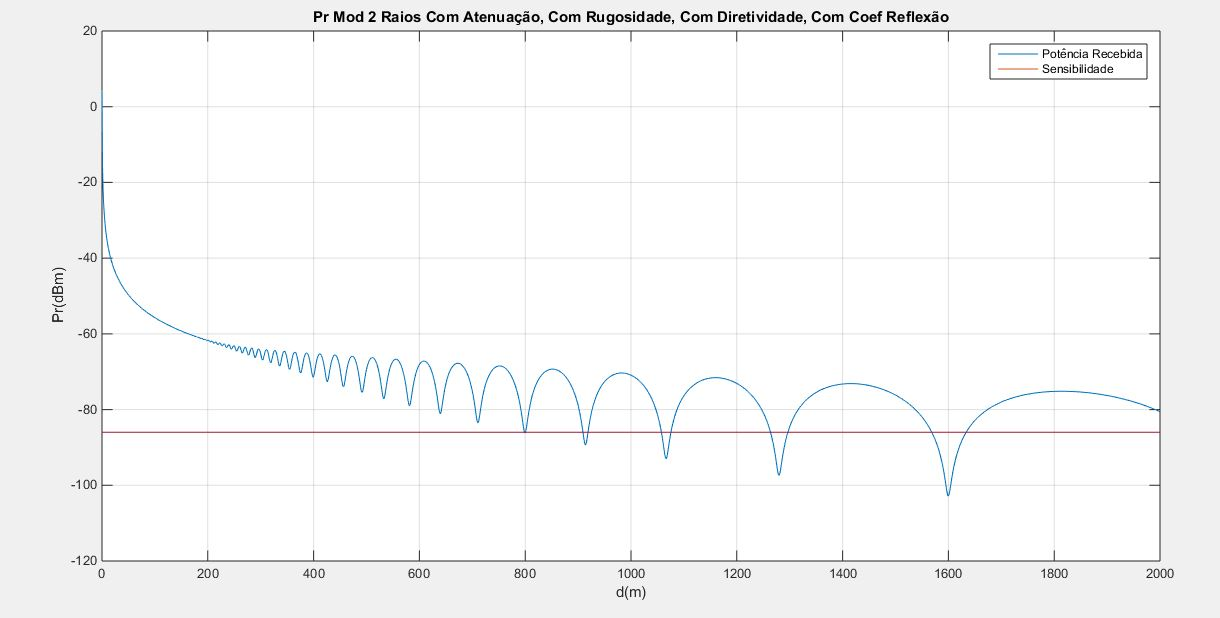
\includegraphics[scale = 0.3]{Figuras/Pr_h_20_1.JPG}
\caption{Potência Recebida na antena receptora, estando as antenas a mesma altura de 20m do solo, com atenuação, com rugosidade, com diretividade e com coeficiente de reflexão.}
\end{figure}
\FloatBarrier

\FloatBarrier
\begin{figure}[!htp]
\centering
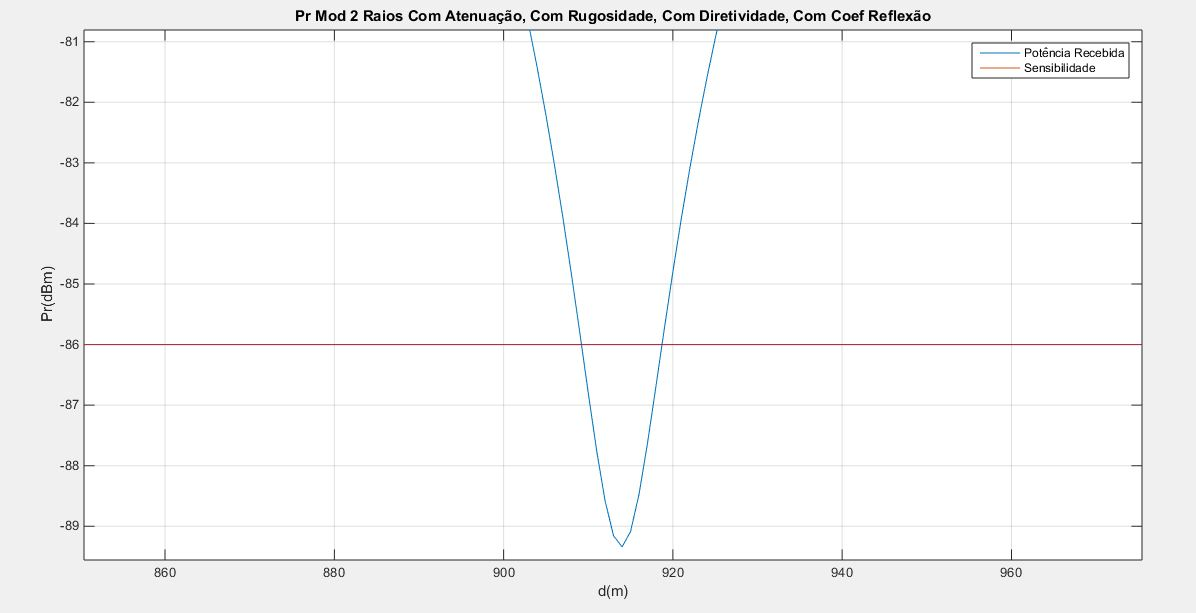
\includegraphics[scale = 0.3]{Figuras/Pr_h_20__2.JPG}
\caption{Potência Recebida na antena receptora, estando as antenas a mesma altura de 20m do solo, com atenuação, com rugosidade, com diretividade e com coeficiente de reflexão, abaixo da sensibilidade pela primeira vez.}
\label{h20}
\end{figure}

\FloatBarrier

\paragraph{}A figura \ref{h20} mostra que a distância ótima para o enlace é  $d \approx 910m$, o que já é uma vantagem em relação a altura de 40m das antenas analisadas a priori.


\paragraph{}Portanto, o melhor cenário para o dimensionamento do enlace é o cenário em que as antenas, transmissora e receptora, apresentam a mesma altura, e a menor possível. 
\chapter{Conclusão}
\paragraph{} Não foi possível até a data de entrega deste relatório à banca examinadora, realizar testes com o sistema completo. Porém em testes preliminares e simulações foi possível averiguar os parâmetros para o funcionamento do sistema. 

\paragraph{} Quanto a sua interface o sistema proposto foi validado em sistema operacional Windows 10, Linux Ubuntu 16.04 e Raspbian. Em todos os sistemas a placa foi detectada com sucesso e o \textit{driver} do sistema instalou um interface de rede ligada ao dispositivo.

\paragraph{} Quanto a transmissão de pacotes em canal RF com antena de polarização vertical omnidirecional com 2,5 dBi de ganho, o sistema foi testado para um alcance de 1km em ambiente urbano.

\paragraph{} Dessa forma podemos concluir que para causo de uso proposto como demanda do projeto, (até 15 VANTs com computador de bordo Linux em voo com altura variável de 40 a 60 metros espalhados em uma área de até 500 metros da base) o sistema desenvolvido atende, até então, ao que foi solicitado com prejuízo da conexão dos modems em rede descentralizada objetivo que está em estágio avançado de implementação.

\paragraph{} Ao longo do desenvolvimento do projeto foram encontrados diverso desafios que acabaram por atrasar o cronograma do projeto. Entre esses desafios podemos citar a implementação da classe USB no microcontrolador utilizado no projeto, que se tornou uma etapa de difícil depuração devido a conflitos de segurança de baixo nível do SO utilizado na depuração, também podemos citar a decodificação do sinal em RDS, que torna necessária a demodulação exata do sinal e reversão de todas as etapas de codificação de forma a obter o pacote \textit{ethernet} original.

\paragraph{}Quanto a escolha das antenas a serem utilizadas, depois do dimensionamento do enlace, utilizando o Modelo de 2 Raios como modelo teórico, chegamos a conclusão que a situação ideal para o sistema exige um cenário no qual os VANTs devem estar voando à uma mesma altura, para que a potência recebida na antena receptora será a maior possível, em comparação a outros cenários em que os VANTs voam em alturas distintas. 

\paragraph{}Considerando, assim que as antenas estejam a uma mesma altura do solo, chegou-se a conclusão de que as antenas deveriam estar voando a menor altura possível, $h_t = h_r = 20m$, de forma a otimizar o desempenho do enlace, apresentando, assim, uma distância máxima de funcionamento sem perda de informação de $d \approx 910m$. 

% -----
% PARTE DE REFERÊCIAS BIBLIOGRÁFICAS DE PFC
%
%  As referências do documento de PFC devem estar no arquivo refs.bib
%  Devem seguir o formato bibtex - ver Manual-Referencias.pdf para mais detalhes.
% -----
\bibliographystyle{pfc}
\bibliography{refs}

% -----
% PARTE DE APÊNDICE DE PFC
%
%  Se o documento de PFC não tiver apêndices REMOVER AS LINHAS ABAIXO
%  Adicionar os arquivos .tex de apêndice ao documento com comando \include{•}
% -----
%\inappendix
%%%
%
% ARQUIVO: apendice.tex
%
% VERSÃO: 1.0
% DATA: Maio de 2016
% AUTOR: Coordenação de Trabalhos Especiais SE/8
% 
%  Arquivo tex de exemplo de apêndice do documento de Projeto de Fim de Curso.
%  Este exemplo traz dois apêndices (dois comandos \chapter{•}). Poderiam ser colocados em arquivos .tex
%  separados. Neste caso, o arquivo main.tex deveria ter um \include{•} para cada arquivo .tex
%
% ---
% DETALHES
%  a. todo apêndice deve começar com \chapter{•}
%  b. usar comando \noindent logo após \chapter{•}
%  c. segue os mesmos DETALHES do arquivo .tex de exemplo de capítulo do documento de Projeto de Fim de Curso
% ---
%%
\chapter{Apêndice Exemplo}
\noindent
Curabitur tortor. Pellentesque nibh. Aenean quam. In scelerisque sem at dolor. Maecenas mattis. Sed convallis tristique sem. Proin ut ligula vel nunc egestas porttitor. Morbi lectus risus, iaculis vel, suscipit quis, luctus non, massa. Fusce ac turpis quis ligula lacinia aliquet. Mauris ipsum. Nulla metus metus, ullamcorper vel, tincidunt sed, euismod in, nibh. Quisque volutpat condimentum velit.

Class aptent taciti sociosqu ad litora torquent per conubia nostra, per inceptos himenaeos. Nam nec ante. Sed lacinia, urna non tincidunt mattis, tortor neque adipiscing diam, a cursus ipsum ante quis turpis. Nulla facilisi. Ut fringilla. Suspendisse potenti. Nunc feugiat mi a tellus consequat imperdiet. Vestibulum sapien. Proin quam. Etiam ultrices. Suspendisse in justo eu magna luctus suscipit. Sed lectus. Integer euismod lacus luctus magna.

Lorem ipsum dolor sit amet, consectetur adipiscing elit. Integer nec odio. Praesent libero. Sed cursus ante dapibus diam. Sed nisi. Nulla quis sem at nibh elementum imperdiet. Duis sagittis ipsum. Praesent mauris. Fusce nec tellus sed augue semper porta. Mauris massa. Vestibulum lacinia arcu eget nulla. Class aptent taciti sociosqu ad litora torquent per conubia nostra, per inceptos himenaeos. Curabitur sodales ligula in libero. Sed dignissim lacinia nunc.

\chapter{Apêndice Exemplo 02}
\noindent
Curabitur tortor. Pellentesque nibh. Aenean quam. In scelerisque sem at dolor. Maecenas mattis. Sed convallis tristique sem. Proin ut ligula vel nunc egestas porttitor. Morbi lectus risus, iaculis vel, suscipit quis, luctus non, massa. Fusce ac turpis quis ligula lacinia aliquet. Mauris ipsum. Nulla metus metus, ullamcorper vel, tincidunt sed, euismod in, nibh. Quisque volutpat condimentum velit.

Class aptent taciti sociosqu ad litora torquent per conubia nostra, per inceptos himenaeos. Nam nec ante. Sed lacinia, urna non tincidunt mattis, tortor neque adipiscing diam, a cursus ipsum ante quis turpis. Nulla facilisi. Ut fringilla. Suspendisse potenti. Nunc feugiat mi a tellus consequat imperdiet. Vestibulum sapien. Proin quam. Etiam ultrices. Suspendisse in justo eu magna luctus suscipit. Sed lectus. Integer euismod lacus luctus magna.

Lorem ipsum dolor sit amet, consectetur adipiscing elit. Integer nec odio. Praesent libero. Sed cursus ante dapibus diam. Sed nisi. Nulla quis sem at nibh elementum imperdiet. Duis sagittis ipsum. Praesent mauris. Fusce nec tellus sed augue semper porta. Mauris massa. Vestibulum lacinia arcu eget nulla. Class aptent taciti sociosqu ad litora torquent per conubia nostra, per inceptos himenaeos. Curabitur sodales ligula in libero. Sed dignissim lacinia nunc.

%\outappendix

% -----
% PARTE DE ANEXO DE PFC
%
%  Se o documento de PFC não tiver anexos REMOVER AS LINHAS ABAIXO
%  Adicionar os arquivos .tex de anexo ao documento com comando \include{•}
% -----
%\inannex
%%%
%
% ARQUIVO: anexo.tex
%
% VERSÃO: 1.0
% DATA: Maio de 2016
% AUTOR: Coordenação de Trabalhos Especiais SE/8
% 
%  Arquivo tex de exemplo de anexo do documento de Projeto de Fim de Curso.
%  Este exemplo traz dois anexos (dois comandos \chapter{•}). Poderiam ser colocados em arquivos .tex
%  separados. Neste caso, o arquivo main.tex deveria ter um \include{•} para cada arquivo .tex
%
% ---
% DETALHES
%  a. todo anexo deve começar com \chapter{•}
%  b. usar comando \noindent logo após \chapter{•}
%  c. segue os mesmos DETALHES do arquivo .tex de exemplo de capítulo do documento de Projeto de Fim de Curso
% ---
%%
\chapter{Anexo Exemplo}
\noindent
Id magna feugiat. Erat pellentesque sapien in rhoncus dolor augue vel eget. Erat nibh animi ultricies sit rhoncus. Eleifend aliquam luctus sem turpis habitasse. Lectus arcu ut mi nulla luctus facilisis cursus suspendisse class sociis metus vitae leo consequat lorem ullamcorper arcu. Nunc justo aliquam. Quidem volutpat urna. Nonummy nulla blandit donec vitae ultrices. Netus aliquam vivamus. Vehicula libero leo. Vestibulum consectetuer magna. Sapien aliquam arcu netus etiam lectus. Venenatis tristique morbi non nulla tortor commodo gravida ac neque lacinia urna. Elit mauris adipisci. Vitae sed curabitur. Tellus nunc lectus. Nonummy et integer.

Lorem dictumst enim. Dui vestibulum quisque. Dolor posuere risus. Nullam vitae est magnis est tortor metus dolor integer. Massa elit nec euismod et lacus quam ac malesuada est suspendisse ut est pellentesque vivamus lorem amet non vulputate maecenas et id ultrices lacus odio morbi vitae ac aenean in feugiat elit sodales congue proin dui leo bibendum scelerisque faucibus in suscipit. Nulla parturient in. Eget habitasse fringilla. Eget donec excepturi wisi lorem lacinia. Elementum lorem sem. Pede metus sit. Aenean facilisi pellentesque. Purus dictum ante. Neque amet sed.

Sed leo molestie. Elit fusce placerat lectus quis aliquam nulla turpis platea. Integer mus bibendum sed wisi pretium ullamcorper nunc arcu. Ipsum maecenas sed. Et pariatur in. Ut wisi non. Bibendum nec et quisque quam diam sed dolor lorem. Pellentesque fames donec senectus nulla purus dui nibh praesent. Pariatur nulla augue sapien elit imperdiet aliquam ullamcorper orci. Integer nec mauris. Sit magnis vel ut leo a sapien proin at. Etiam sem aliquam bibendum mauris purus ac sagittis ultrices. Mollis eleifend est. Nec vitae posuere at arcu purus. In elementum vehicula.

\chapter{Anexo Exemplo 02}
\noindent
Id magna feugiat. Erat pellentesque sapien in rhoncus dolor augue vel eget. Erat nibh animi ultricies sit rhoncus. Eleifend aliquam luctus sem turpis habitasse. Lectus arcu ut mi nulla luctus facilisis cursus suspendisse class sociis metus vitae leo consequat lorem ullamcorper arcu. Nunc justo aliquam. Quidem volutpat urna. Nonummy nulla blandit donec vitae ultrices. Netus aliquam vivamus. Vehicula libero leo. Vestibulum consectetuer magna. Sapien aliquam arcu netus etiam lectus. Venenatis tristique morbi non nulla tortor commodo gravida ac neque lacinia urna. Elit mauris adipisci. Vitae sed curabitur. Tellus nunc lectus. Nonummy et integer.

Lorem dictumst enim. Dui vestibulum quisque. Dolor posuere risus. Nullam vitae est magnis est tortor metus dolor integer. Massa elit nec euismod et lacus quam ac malesuada est suspendisse ut est pellentesque vivamus lorem amet non vulputate maecenas et id ultrices lacus odio morbi vitae ac aenean in feugiat elit sodales congue proin dui leo bibendum scelerisque faucibus in suscipit. Nulla parturient in. Eget habitasse fringilla. Eget donec excepturi wisi lorem lacinia. Elementum lorem sem. Pede metus sit. Aenean facilisi pellentesque. Purus dictum ante. Neque amet sed.

Sed leo molestie. Elit fusce placerat lectus quis aliquam nulla turpis platea. Integer mus bibendum sed wisi pretium ullamcorper nunc arcu. Ipsum maecenas sed. Et pariatur in. Ut wisi non. Bibendum nec et quisque quam diam sed dolor lorem. Pellentesque fames donec senectus nulla purus dui nibh praesent. Pariatur nulla augue sapien elit imperdiet aliquam ullamcorper orci. Integer nec mauris. Sit magnis vel ut leo a sapien proin at. Etiam sem aliquam bibendum mauris purus ac sagittis ultrices. Mollis eleifend est. Nec vitae posuere at arcu purus. In elementum vehicula.

%\outannex

% -----
% FIM DO DOCUMENTO DE PFC
% -----
\label{theend}
\end{document}
